\documentclass[11pt]{beamer}

% \usetheme{CambridgeUS}
% \usecolortheme{dolphin}
\usepackage{amsmath}
\usepackage{amssymb}
\usepackage{amsfonts}

\usepackage{algorithm}
%\usepackage{algorithmic}
\usepackage{algorithmicx}
\usepackage{algpseudocode}

\usepackage{hyperref}
\usepackage[utf8]{inputenc}

\usepackage{graphicx}
\graphicspath{{./figures/}}
\usepackage[english]{babel}

\usepackage{url}
\usepackage{color}
\usepackage{xcolor}

\usepackage{tcolorbox}
\usepackage{minted}

\usepackage{mdframed}
\usepackage{tikz}


\usefonttheme[onlymath]{serif}

\hypersetup{
  colorlinks,
  citecolor=green,
  linkcolor=black
}

\definecolor{darkgreen}{RGB}{0,128,0}
 
\hypersetup{
  colorlinks,
  citecolor=darkgreen,
  linkcolor=black
}

\usepackage{natbib}

\title{Introduction to Neural Networks for Molecular Graphs}
%\subtitle{ Inspired from \cite{raschka2022machine, chollet2021deep,
 %   geron2022hands}}

\author{Benoit Gaüzère}


\def\dbR{{\mathrm{I\hskip-2.2pt R}}}
\def\dbN{{\mathrm{I\hskip-2.2pt N}}}
\def\esp{{\mathrm{I\hskip-1.5pt E}}}
\def\pr{{\mathrm{I\hskip-2.2pt P}}}
\def\halam{{\widehat{\lambda}}}
\def\hasig{{\widehat{\sigma}}}
\def\hae{{\widehat{\varepsilon}}}
\def\tQ{{\widehat{Q}}}

\def\tR{{\widehat{R}}}
\def\halpha{{\widehat{\alpha}}}
\def\haa{{\widehat{a}}}
\def\ha{{\widehat{a}}}
\def\he{{\widehat{\varepsilon}}}
\def\hb{{\widehat{b}}}
\def\hab{{\widehat{b}}}
\def\haE{{\widehat{E}}}
\def\hsigma{{\widehat{\sigma}}}
\def\hay{{z}}
\def\baR{{\overline{R}}}
\def\baE{{\overline{E}}}
\def\baX{{\overline{X}}}
\def\bax{{\overline{x}}}
\def\baY{{\overline{Y}}}
\def\bay{{\overline{y}}}
\def\barY{{\overline{Y}}}
\def\mx{{\overline{x}}}
\def\my{{\overline{y}}}
\def\lamMV{{\widehat{\lambda}_{MV}}}
\def\lamef{{\widehat{\lambda}_{e}}}

%\def\dbC{{\mathrm{I\hskip-5.4pt C}}}
\def\dbC{{\mathds{C}}}
\def\un{{\mathds{1}}}
\def\a{{\mathrm{a}}}
\def\b{{\mathrm{b}}}
\def\bc{{\mathrm{c}}}
\def\d{{\boldsymbol{d}}}
\def\e{{\mathrm{e}}}
\def\m{{\mathrm{m}}}
\def\n{{\mathrm{n}}}
\def\p{{\mathrm{p}}}
\def\r{{\mathrm{r}}}
\def\s{{\mathrm{s}}}
\def\u{{\mathrm{u}}}
\def\v{{\mathrm{v}}}
\def\ones{{\boldsymbol{\mathbb{1}}}}
\def\w{{\boldsymbol{w}}}
\def\x{{\mathbf{x}}}
\def\X{{\boldsymbol{X}}}
\def\y{{\boldsymbol{y}}}
\def\z{{\boldsymbol{z}}}
\def\tx{{\widetilde{x}}}
\def\bPhi{{\mathrm{\Phi}}}
\def \habeta{{\widetilde{\beta}}}
\def\Cmat{{\boldsymbol{C}}}

\def\tL{{\widetilde{L}}}
\def\tF{{\widetilde{F}}}
\def\tM{{\widetilde{M}}}
\def\tH{{\widetilde{H}}}
\def\tD{{\widetilde{D}}}
\def\tU{{\widetilde{U}}}
\def\vh{{\bar{v}^\top}}
\def\det{{\mbox{det}}}
\def\atimes{{\alert{\times}}}

\def\clO{{\mathcal{O}}}
\def\clA{{\mathcal{A}}}
\def\clB{{\mathcal{B}}}
\def\clD{{\mathcal{D}}}
\def\clL{{\mathcal{L}}}
\def\clN{{\mathcal{N}}}
\def\clH{{\mathcal{H}}}
\def\clT{{\mathcal{T}}}
\def\clY{\mathcal{Y}}
\def\fl{{\mbox{fl}}}

%\input{notation}

%%%%%%%%%%%%%%%%%%%%%%%%%%%%%%%%%%%%%%%%%%%%%%%%%%%%%%%%%%
\def\dbC{{\mathrm{I\hskip-4.7pt C}}}
\def\dbR{{\mathrm{I\hskip-2.2pt R}}}
\def\un{{\mathrm{I\hskip-5.9pt 1}}}
\def\dbN{{\mathrm{I\hskip-2.2pt N}}}
\def\esp{{\mathrm{I\hskip-1.5pt E}}}
\def\pr{{\mathrm{I\hskip-2.2pt P}}}
\def\hpr{\widehat{\mathrm{I\hskip-2.2pt P}}}
%\def\balpha{{\mathbf{\alpha}}}
\def\a{{\mathbf{a}}}
\def\b{{\mathbf{b}}}
\def\bc{{\mathbf{c}}}
%\def\d{{\mathbf{d}}}
\def\e{{\mathbf{e}}}
\def\f{{\mathbf{f}}}
\def\g{{\mathbf{g}}}
\def\h{{\mathbf{h}}}
\def\p{{\mathbf{p}}}
\def\q{{\mathbf{q}}}
\def\u{{\mathbf{u}}}
\def\v{{\mathbf{v}}}
%def\x{{\mathbf{x}}}
\def\xb{{\overline{x}}}
\def\yb{{\overline{y}}}
%\def\w{{\mathbf{w}}}
\def\haF{{\widehat{F}}}
\def\hap{{\widehat{p}}}
\def\R{\mathbb{R}}
\def\P{\mathbb{P}}
\def\E{\mathbb{E}}
\def\bX{\mathbb{X}}
\def\haF{{\widehat{F}}}
\def\haf{{\widehat{f}}}
\def\ham{{\widehat{m}}}
\def\haM{{\widehat{M}}}
\def\hamu{{\widehat{\mu}}}
\def\hasigma{{\widehat{\sigma}}}
\def\hap{{\widehat{\pr}}}
\def\haphi{{\widehat{\phi}}}
\def\haS{{\widehat{S}}}
\def\has{{\widehat{s}}}
\def\haQ{{\widehat{Q}}}
\def\hamc{{\widehat{mc}}}
\def\barX{{\bar{X}}}
\def\barx{{\bar{x}}}
\def\bary{{\bar{y}}}
\def\haPr{{\widehat{\mathrm{I\hskip-2.2pt P}}}}
\def\hap{{\widehat{p}}}
\def\bmu{{\boldsymbol{\mu}}}
\def\point{{\mbox{\tiny\textbullet}}}

%%%%%%%%%%%%%%%%%%%%%%%%%%%%%%%%%%%%%%%%%%%%%%%%%%%%%%%%%%%%%%%%%%%%%%%%%%%%%%%%%%%%%%%%%%%%%%%%%%%%%%%%%%%%%%%%%%%%%%%%%%%%
%%%%%%%%%%%%%%%%%%%%%%%%%%%%%%%%%%%%%%%%%%%%%%%%%%%%%%%%%%%%%%%%%%%%%%%%%%%%%%%%%%%%%%%%%%%%%%%%%%%%%%%%%%%%%%%%%%%%%%%%%%%%

\def\dbR{{\mathrm{I\hskip-2.2pt R}}}
\def\dbN{{\mathrm{I\hskip-2.2pt N}}}
\def\esp{{\mathrm{I\hskip-1.5pt E}}}
\def\pr{{\mathrm{I\hskip-2.2pt P}}}
\def\halam{{\widehat{\lambda}}}
\def\hasig{{\widehat{\sigma}}}
\def\tQ{{\widehat{Q}}}

\def\tR{{\widehat{R}}}
\def\haa{{\widehat{a}}}
\def\hab{{\widehat{b}}}
\def\haE{{\widehat{E}}}
\def\baR{{\overline{R}}}
\def\baE{{\overline{E}}}
\def\baX{{\overline{X}}}
\def\baY{{\overline{Y}}}
\def\lamMV{{\widehat{\lambda}_{MV}}}
\def\lamef{{\widehat{\lambda}_{e}}}
\def\k{{\mathnormal{k}}}
\def\f{{\mathnormal{f}}}
\def\g{{\mathnormal{g}}}
\def\datax{{\mathnormal{x}}}
\def\K{{\mathbf{K}}}
\def\G{{\mathbf{G}}}

%\def\dbC{{\mathrm{I\hskip-5.4pt C}}}
\def\dbC{{\mathds{C}}}
\def\un{{\mathds{1}}}
\def\a{{\mathbf{a}}}
\def\b{{\mathbf{b}}}
\def\c{{\mathbf{c}}}
%\def\d{{\mathbf{d}}}
\def\e{{\mathbf{e}}}
\def\m{{\mathbf{m}}}
\def\p{{\mathbf{p}}}
\def\r{{\mathbf{r}}}
\def\u{{\mathbf{u}}}
\def\v{{\mathbf{v}}}
%\def\w{{\mathbf{w}}}

\def\Un{{\mathrm{{1\hskip-2.6pt I}}}}

\def\dist{{d_m}}

\def\t{{\mathbf{t}}}
\def\s{{\mathbf{s}}}
%def\x{{\mathbf{x}}}

\def\tx{{\widetilde{x}}}
\def\tL{{\widetilde{L}}}
\def\tF{{\widetilde{F}}}
\def\tM{{\widetilde{M}}}
\def\tH{{\widetilde{H}}}
\def\ttau{{\widetilde{\tau}}}
\def\tD{{\widetilde{D}}}
\def\tU{{\widetilde{U}}}
\def\vh{{\bar{v}^\top}}
\def\det{{\mbox{det}}}
\def\atimes{{\alert{\times}}}

\def\balpha{{\boldsymbol\alpha}}
\def\bbeta{{\boldsymbol\beta}}
\def\clO{{\mathcal{O}}}
\def\clA{{\mathcal{A}}}
\def\clL{{\mathcal{L}}}
\def\clQ{{\mathcal{Q}}}
\def\clD{{\mathcal{D}}}
\def\clX{{\mathcal{X}}}
\def\clH{{\mathcal{H}}}
\def\clY{{\mathcal{Y}}}
\def\clP{{\mathcal{P}}}
\def\clS{{\mathcal{S}}}
\def\bfX{{\mathbf{X}}}
\def\bfB{{\mathbf{B}}}
\def\bfA{{\mathbf{A}}}

\def\bfI{{\mathbf{I}}}
\def\fl{{\mbox{fl}}}

\def\R{{\mathbb{N}}}
\def\R{{\mathbb{R}}}
\def\0{{\mathbf{0}}}
\def\1{{\mathbb{1}}}
\DeclareMathOperator*{\argmin}{argmin}
\DeclareMathOperator*{\argmax}{argmax} 
\DeclareMathOperator*{\mymin}{min}
\DeclareMathOperator*{\mymax}{max}
\RequirePackage{bbold}
\RequirePackage{kvoptions}

\newcommand{\complex}[1]{\mbox{$\mathcal{O}(#1)$}}
\newcommand{\cluster}[1]{\mbox{$\mathcal{C}_{#1}$}}


\def\T{{\mathsf{T}}}
\newcommand\dangersign[1][2ex]{%
  \renewcommand\stacktype{L}%
  \scaleto{\stackon[1.3pt]{\color{red}$\triangle$}{\tiny !}}{#1}%
}
\renewcommand{\vec}[1]{\mathbf{#1}}


\DeclareMathOperator*{\triinf}{\tt tri\_inf}
\DeclareMathOperator*{\diag}{\tt diag}

\newcommand{\Perm}[2]{P_{#1 \leftrightarrow #2}}
\DeclareMathOperator*{\triinfunit}{\tt tri\_inf\_unit}
\DeclareMathOperator*{\triangularise}{\tt factorisation\_LU}
\DeclareMathOperator*{\factopalu}{\tt factorisation\_PALU}
\DeclareMathOperator*{\factoldm}{\tt factorisation\_LDM}
\DeclareMathOperator*{\factoldl}{\tt factorisation\_LDL}
\DeclareMathOperator*{\factochol}{\tt Cholesky}
\DeclareMathOperator*{\factocholrec}{\tt Cholesky\_Rec}
\DeclareMathOperator*{\factocholinc}{\tt Cholesky\_Incr}
\DeclareMathOperator*{\trisup}{\tt tri\_sup}
\DeclareMathOperator*{\tfgauss}{\tt Tf\_Gauss}
\DeclareMathOperator*{\gausselim}{\tt Gauss\_Elimination}
\DeclareMathOperator*{\mettreajour}{\tt mettre\_a\_jour}
\DeclareMathOperator*{\triu}{\tt triu}
\DeclareMathOperator*{\assign}{\leftarrow}
\DeclareMathOperator*{\resolve}{\tt resoud}
\DeclareMathOperator*{\swap}{\leftrightarrow}
\newenvironment{rcases} 
        {\left.\begin{aligned}}
         {\end{aligned}\hspace{0.5cm}\right\rbrace}

% \renewenvironment{definition}[1]
% {
%   \begin{mdframed}[backgroundcolor=blue]
%     \textbf{Définition : #1}\\
%     \setlength{\alglength}{.95\linewidth} \begin{minipage}[t]{\alglength}
% }{        \end{minipage}
%     % \end{algorithmfloat}
%   \end{mdframed}
% }
\renewcommand{\emph}[1]{{\color{blue} #1}}
\renewenvironment{definition}[1][]{%                                                                         
  \ifstrempty{#1}%                                                                                   
  {\mdfsetup{%                                                                                       
    frametitle={%                                                                                    
      \tikz[baseline=(current bounding box.east),outer sep=0pt]                                     
       \node[anchor=east,rectangle,fill=blue!20]                                                    
        {\strut Définition};}}                                                                 
  }%                                                                                                 
  {\mdfsetup{%                                                                                       
      frametitle={%                                                                                   
        \tikz[baseline=(current bounding box.east),outer sep=0pt]                                     
        \node[anchor=east,rectangle,fill=blue!20]                                                    
        {\strut Définition~:~#1};}}%                                                            
  }%                                                                                                
  \mdfsetup{innertopmargin=10pt,linecolor=blue!20,%                                                 
    linewidth=2pt,topline=true,                                                             
    frametitleaboveskip=\dimexpr-\ht\strutbox\relax,}                                       
  \begin{mdframed}[]\relax%                                                                         
  }{\end{mdframed}}                                                                                 

\renewenvironment{lemma}[1][]{%                                                                         
  \ifstrempty{#1}%                                                                                   
  {\mdfsetup{%                                                                                       
    frametitle={%                                                                                    
      \tikz[baseline=(current bounding box.east),outer sep=0pt]                                     
       \node[anchor=east,rectangle,fill=green!10]                                                    
        {\strut Lemme};}}                                                                 
  }%                                                                                                 
  {\mdfsetup{%                                                                                       
      frametitle={%                                                                                   
        \tikz[baseline=(current bounding box.east),outer sep=0pt]                                     
        \node[anchor=east,rectangle,fill=green!10]                                                    
        {\strut Lemme~:~#1};}}%                                                            
  }%                                                                                                
  \mdfsetup{innertopmargin=10pt,linecolor=green!10,%                                                 
    linewidth=2pt,topline=true,                                                             
    frametitleaboveskip=\dimexpr-\ht\strutbox\relax,}                                       
  \begin{mdframed}[]\relax%                                                                         
  }{\end{mdframed}}                                                                                 

\renewenvironment{theorem}[1][]{%                                                                         
  \ifstrempty{#1}%                                                                                   
  {\mdfsetup{%                                                                                       
    frametitle={%                                                                                    
      \tikz[baseline=(current bounding box.east),outer sep=0pt]                                     
       \node[anchor=east,rectangle,fill=green!50]                                                    
        {\strut Théorème};}}                                                                 
  }%                                                                                                 
  {\mdfsetup{%                                                                                       
      frametitle={%                                                                                   
        \tikz[baseline=(current bounding box.east),outer sep=0pt]                                     
        \node[anchor=east,rectangle,fill=green!50]                                                    
        {\strut Théorème~:~#1};}}%                                                            
  }%                                                                                                
  \mdfsetup{innertopmargin=10pt,linecolor=green!50,%                                                 
    linewidth=2pt,topline=true,                                                             
    frametitleaboveskip=\dimexpr-\ht\strutbox\relax,}                                       
  \begin{mdframed}[]\relax%                                                                         
  }{\end{mdframed}}                                                                                 

\renewenvironment{corollary}[1][]{%                                                                         
  \ifstrempty{#1}%                                                                                   
  {\mdfsetup{%                                                                                       
    frametitle={%                                                                                    
      \tikz[baseline=(current bounding box.east),outer sep=0pt]                                     
       \node[anchor=east,rectangle,fill=green!25]                                                    
        {\strut Corollaire};}}                                                                 
  }%                                                                                                 
  {\mdfsetup{%                                                                                       
      frametitle={%                                                                                   
        \tikz[baseline=(current bounding box.east),outer sep=0pt]                                     
        \node[anchor=east,rectangle,fill=green!25]                                                    
        {\strut Corollaire~:~#1};}}%                                                            
  }%                                                                                                
  \mdfsetup{innertopmargin=10pt,linecolor=green!25,%                                                 
    linewidth=2pt,topline=true,                                                             
    frametitleaboveskip=\dimexpr-\ht\strutbox\relax,}                                       
  \begin{mdframed}[]\relax%                                                                         
  }{\end{mdframed}}                                                                                 


% \newenvironment{theo}[1][]{%
%   \ifstrempty{#1}{
%     \mdfsetup{% 
%       frametitle=%
%       \tikz[baseline =(current bounding box.east)]
%       \node[anchor=east,rectangle,fill=blue!20]
%       {\strut ~Définition};}}
%   {
%     \mdfsetup{%
%       frametitle={%
%         \tikz[baseline=(current bounding box.east)]
%         % \node[anchor=east,rectangle,fill=blue!20]
%         {\strut Définition:~#1};}}%
%   }%
%   \mdfsetup{innertopmargin=10pt,linecolor=blue!20,%
%     linewidth=2pt,topline=true,
%     frametitleaboveskip=\dimexpr-\ht\strutbox\relax,}
%   \begin{mdframed}[]\relax  % 
%   }{
%   \end{mdframed}
% }

\setbeamertemplate{footline}[frame number]
\setbeamertemplate{navigation symbols}{}

\addto\captionsfrench{%
  \renewcommand{\figurename}{Fig.}
}

\def\danger{
\includegraphics[width=0.6cm]{danger}}
\def\bigdanger{
\includegraphics[width=1cm]{danger}}
\def\smalldanger{
\includegraphics[width=.4cm]{danger}}

\def\pn{{\mathnormal{n}}}
\def\pz{{\mathnormal{z}}}
\def\pp{{\mathnormal{p}}}

\def\px{{\mathnormal{x}}}
\def\ps{{\mathnormal{s}}}
\def\pt{{\mathnormal{t}}}

\renewcommand\diag[4]{%
  \multicolumn{1}{p{#2}|}{\hskip-\tabcolsep
  $\vcenter{\begin{tikzpicture}[baseline=0,anchor=south west,inner sep=#1]
  \path[use as bounding box] (0,0) rectangle (#2+2\tabcolsep,\baselineskip);
  \node[minimum width={#2+2\tabcolsep-\pgflinewidth},
        minimum  height=\baselineskip+\extrarowheight-\pgflinewidth] (box) {};
  \draw[line cap=round] (box.north west) -- (box.south east);
  \node[anchor=south west] at (box.south west) {#3};
  \node[anchor=north east] at (box.north east) {#4};
 \end{tikzpicture}}$\hskip-\tabcolsep}}

\newcommand{\blue}[1]{\textcolor{blue}{#1}}
\newcommand{\green}[1]{\textcolor{darkgreen}{#1}}
\newcommand{\arrow}{
   \includegraphics[width=0.5cm]{fleche}
}

\newcommand{\doublearrow}{
  
\includegraphics[width=0.5cm]{flechedouble}
}

\newcommand*{\itemperso}{\includegraphics[width=0.8em]{item}}
\newcommand{\xvec}{\mathbf{x}}
\newcommand{\xiivec}{\mathbf{x_i}}
\newcommand{\xjjvec}{\mathbf{x_j}}
\newcommand{\xpvec}{\mathbf{x'}}
\newcommand{\wvec}{\mathbf{w}}
\newcommand{\betavec}{\mathbf{\beta}}
\newcommand{\alphavec}{\mathbf{\alpha}}
\newcommand{\xivec}{\mathbf{\xi}}


\renewcommand{\complex}[1]{\mbox{$\mathcal{O}(#1)$}}
%\DeclareMathOperator{\dist}{d}
\DeclareMathOperator{\sub}{\# sub}
\DeclareMathOperator{\code}{code}
\DeclareMathOperator{\struct}{struct}
\DeclareMathOperator{\myminimize}{minimize}
\DeclareMathOperator{\mymaximize}{maximize}
\newcommand{\minimiser}[1]{\underset{#1}{\myminimize}}
\newcommand{\maximiser}[1]{\underset{#1}{\mymaximize}}
%\DeclareMathOperator{\mymin}{min}
%\DeclareMathOperator{\mymax}{max}
\newcommand{\vecmath}[1]{\mathbf{#1}}

\newcommand*{\itemplus}{
\includegraphics[width=0.8em]{plus}}
\newcommand*{\itemdanger}{\includegraphics[width=1em]{warning}}
\newcommand*{\itemmoins}{
\includegraphics[width=0.8em]{moins}}

\renewcommand{\H}{\ensuremath{\mathcal{H}}}

\newcommand{\myinf}{
  
\includegraphics[width=0.4cm]{inf}
}
\newcommand{\myinfbar}{
  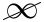
\includegraphics[width=0.4cm]{infbar}
}

\newcommand{\beginbackup}{
   \newcounter{framenumbervorappendix}
   \setcounter{framenumbervorappendix}{\value{framenumber}}
}
\newcommand{\backupend}{
   \addtocounter{framenumbervorappendix}{-\value{framenumber}}
   \addtocounter{framenumber}{\value{framenumbervorappendix}} 
}

\usefonttheme[onlymath]{serif}


\institute{INSA Rouen Normandie - Laboratoire LITIS}

% =================================================================================
\begin{document}
\maketitle

% =================================================================================

\begin{frame}{Outline}
  \tableofcontents
\end{frame}


\section{Introduction}
\subsection{Deep Learning}

\begin{frame}
  \frametitle{The Deep Learning Era}
  \begin{block}{The NN rise}
    Since 2012, we observe the rise of NN based methods :
    \begin{itemize}
    \item Huge datasets
    \item High computationnal capacities (GPU, \dots)
    \item Representation learning $\geq$ handcrafted features
    \end{itemize}
  \end{block}

  \begin{block}{Successes}
    \begin{itemize}
    \item Image/Object recognition
    \item Speech recognition
    \item Natural Language Processing
    \item Game theory (Go)
    \item \dots
    \end{itemize}
  \end{block}
\end{frame}
\subsection{CNN on images}
\begin{frame}
  \frametitle{Deep learning on images : CNN}
  \begin{center}
    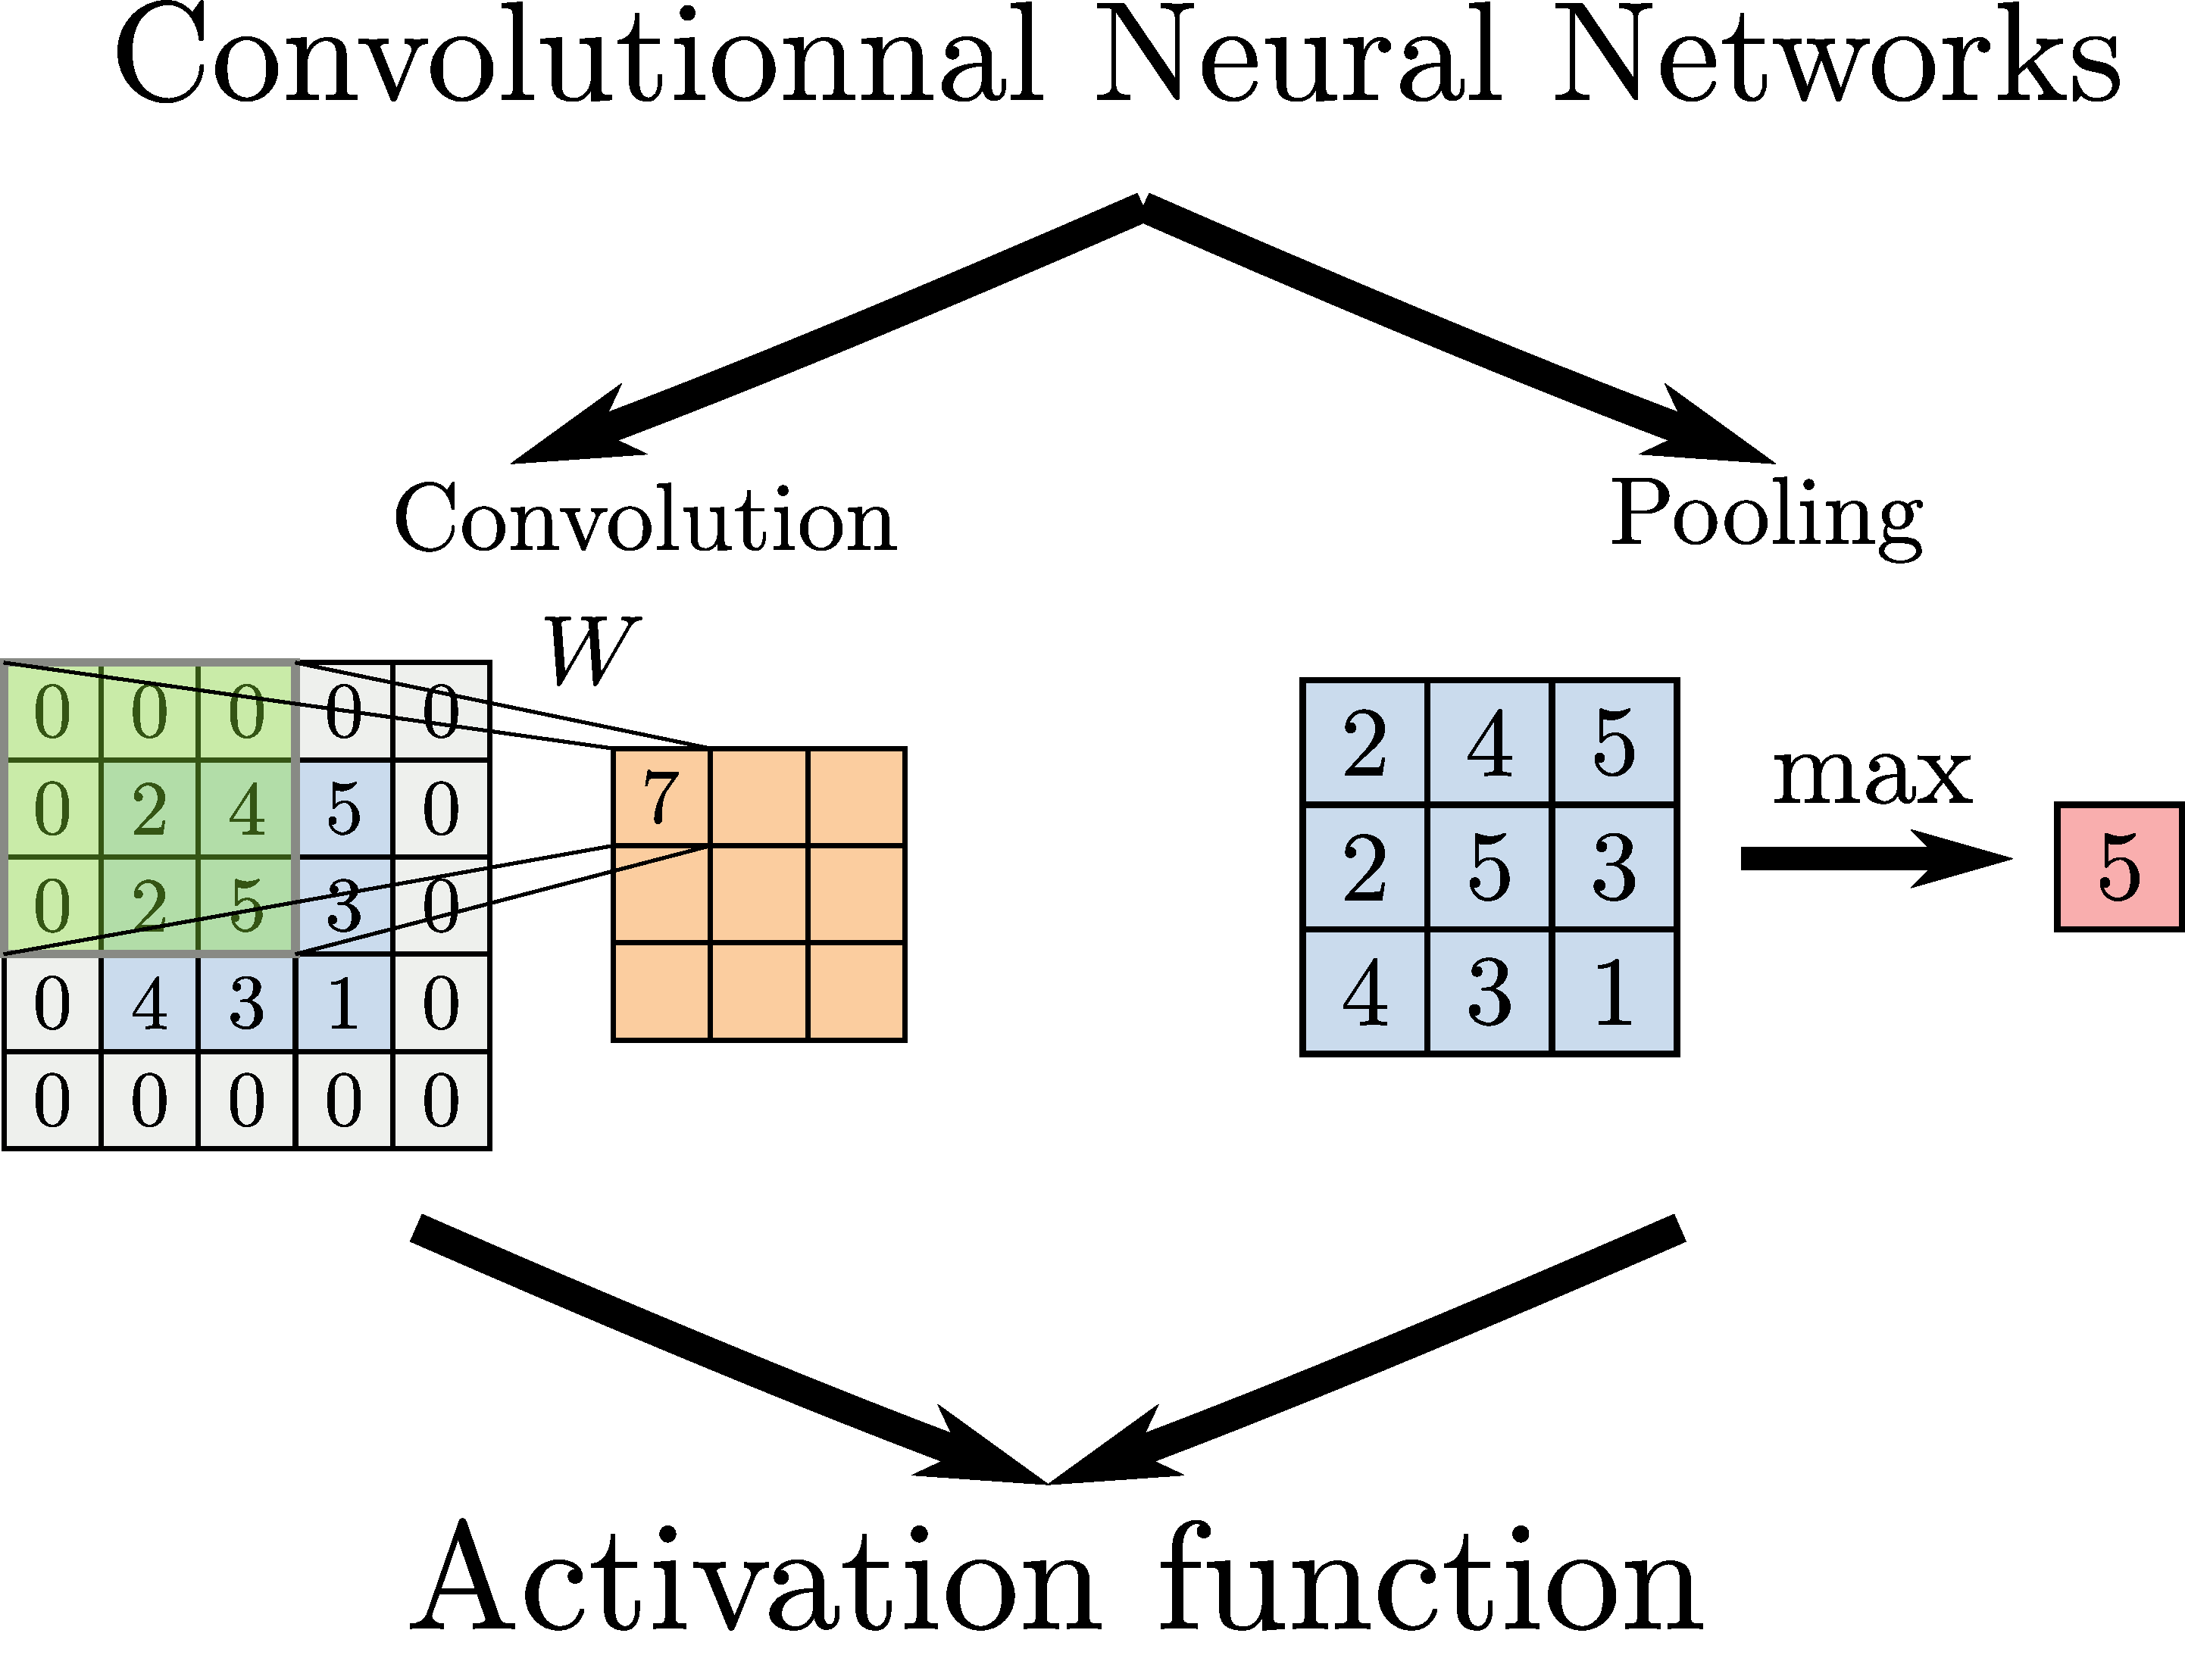
\includegraphics[height=0.75\textheight]{cnn}
  \end{center}
\end{frame}

\begin{frame}{Deep learning on images : CNN}
  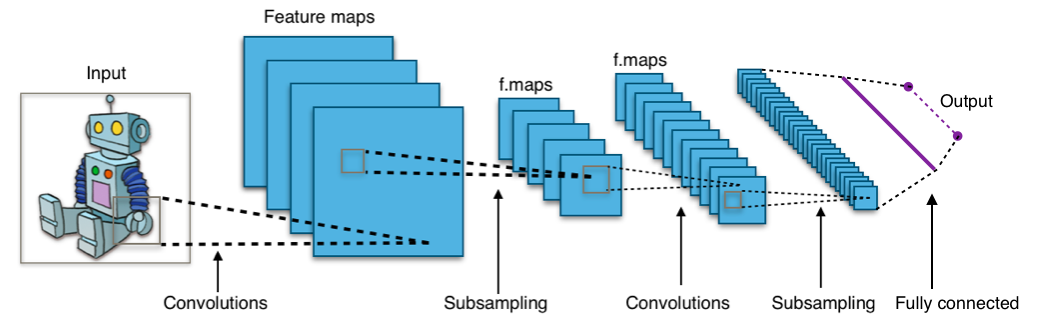
\includegraphics[width=\textwidth]{typical_cnn}
  \flushright{\scriptsize [Wikipedia]}
\end{frame}

\section{Problems on combining graphs and (C)NNs}
\subsection{Non euclidean data}

\begin{frame}{Graph space}
  \begin{block}{What is a graph ?}
    \begin{itemize}
    \item $G = (V, E), E \in V \times V$
    \item Labels :
      \begin{itemize}
      \item $l_v : V \to \dbR^{f_v}$
      \item $l_e : E \to \dbR^{f_e}$
      \end{itemize}
      
    \item degree : $d(v_i) = |\mathcal{N}(v_i)| \in  \dbN^+$
    \item order : $|V|$, size : $|E|$.
    \end{itemize}
    
    
  \end{block}
  \begin{block}{Graph representation (in ML)}
    \begin{itemize}
    \item Adjacency matrix $A \in \{0,1\}^{n \times n}$, with $n =
      |V|$.
      \begin{itemize}
      \item $A(i,j) = 1$ iff. $(v_i,v_j) \in E$
      \end{itemize}
    \item Feature Matrix $X \in \dbR^{n \times f_v}$, $X(i,:)$ $\Rightarrow$
      features of node $v_i$.
    \item Laplacian : $ D - A$, with $D(i,i) = d(v_i)$, else $0$. 
    
    \end{itemize}
  \end{block}
    
\end{frame}

\begin{frame}{Graph space}
  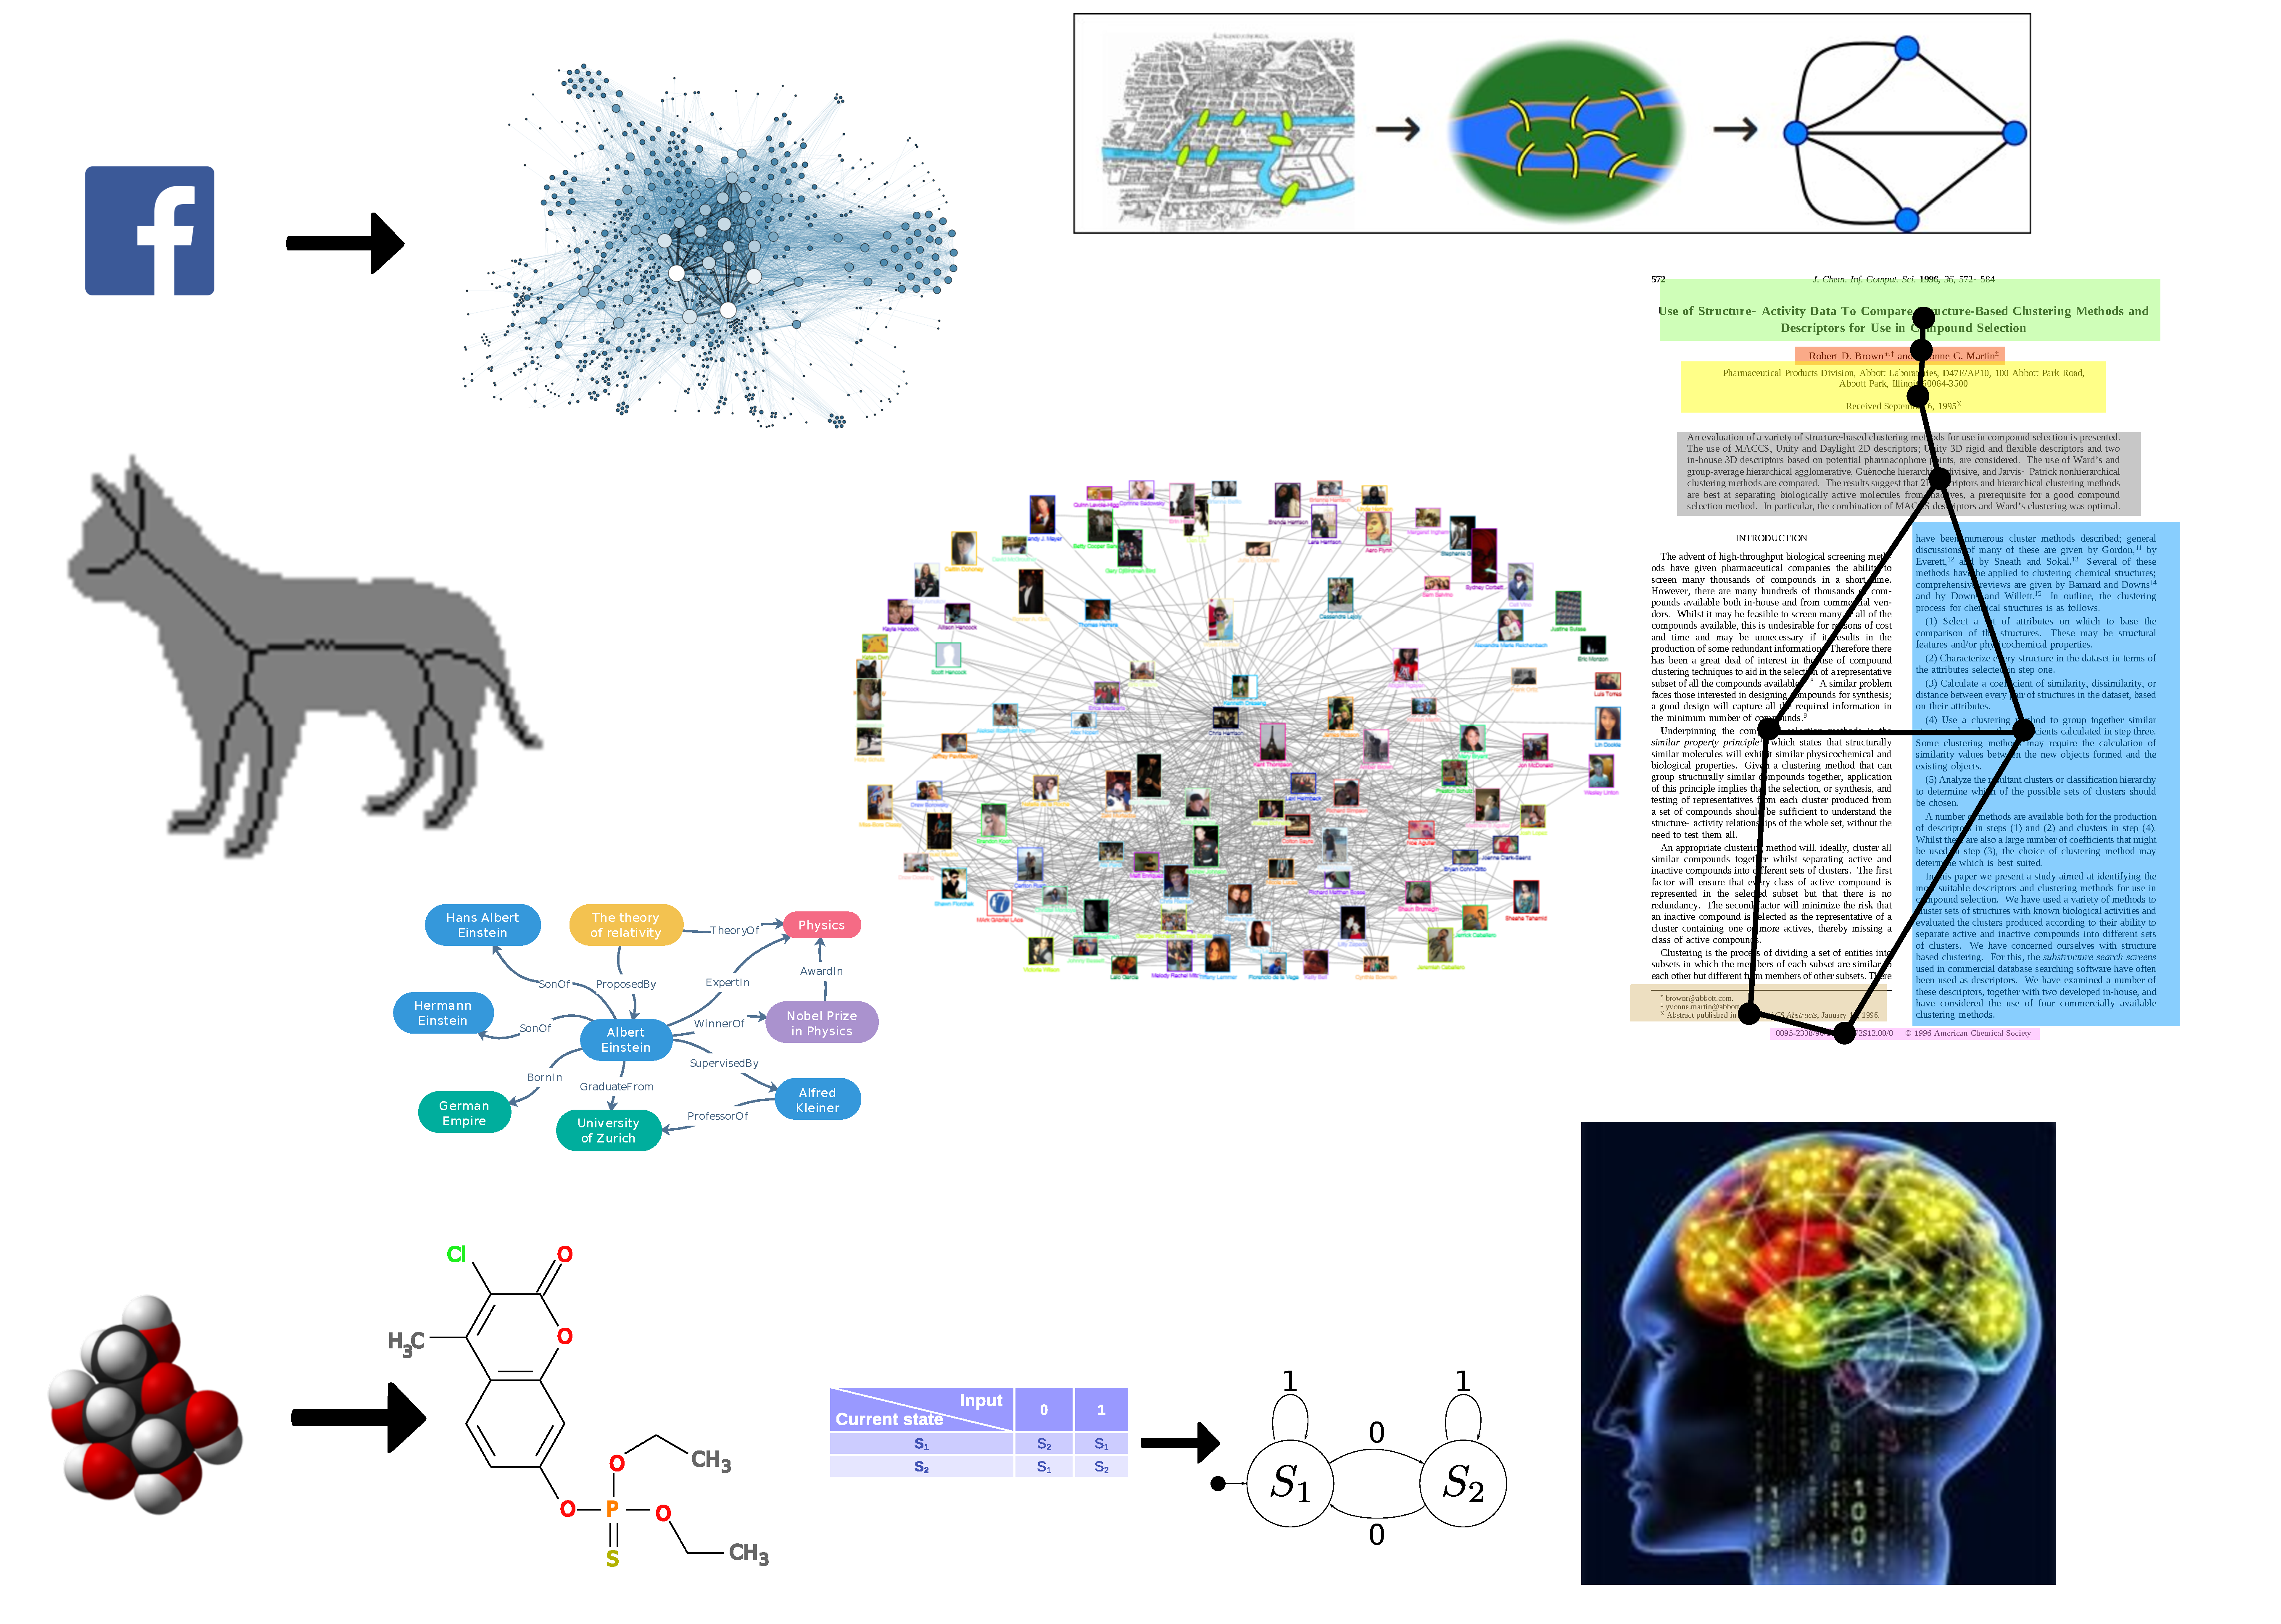
\includegraphics[width=\textwidth]{graph-examples}
  \flushright{{\scriptsize [from Linlin Jia]}}
\end{frame}

\begin{frame}[allowframebreaks]{Tasks on graphs}

  \begin{block}{Node level}
    \begin{itemize}
    \item Node label (i.e. property) prediction
    \begin{itemize}
        \item Regression
        \item Classification
    \end{itemize}
    \item Transductive : predict unlabelled nodes on the same graph
    \item Inductive  : predict node labels on a new graph
    \item Link (labels) prediction
    \item Clustering 
    \end{itemize}
  \end{block}
  \begin{center}
    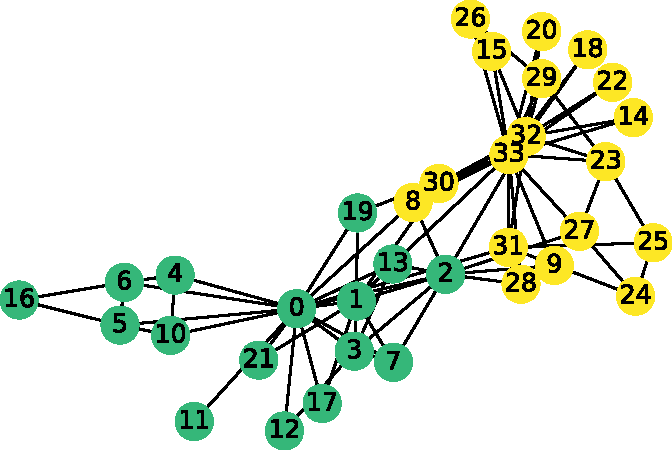
\includegraphics[width=.4\textwidth]{karate}
  \end{center}
  \break
  \begin{block}{Graph level}
    \begin{itemize}
    \item Predict label (i.e. property) for a graph (e.g. toxicity of a molecule)
    \item Graph generation
    \item Metric learning
    \end{itemize}
  \end{block}

  \begin{center}
    \includegraphics[width=.5\textwidth]{graph_level_function}
  \end{center}
    
\end{frame}

\subsection{Graph particularities}

\begin{frame}
  \begin{center}
    \huge {Why ML with graphs is particular ? }
  \end{center}

\end{frame}
\begin{frame}{Graph problems}
  \begin{center}
      \large{Graph space is not an Euclidean space}
    
  \end{center}

  \begin{block}{Variable number of nodes}
    \begin{itemize}
    \item No fixed/limit number of nodes
    \item How to deal with a variable number of nodes/neighbours ? 
    \end{itemize}
  \end{block}

  \begin{block}{Permutation (equi/in)variance}
    \begin{itemize}
    \item No predefined order of nodes
    \item $\Rightarrow$ No order on neighbours ($\neq$ images)
    \end{itemize}
  \end{block}
  
\end{frame}


\begin{frame}{Permutation Invariance}
  \begin{center}
    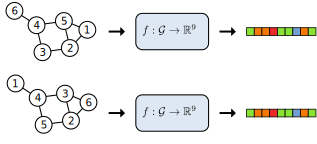
\includegraphics[width=\textwidth]{invariant}
  \end{center}
\end{frame}

\begin{frame}{Permutation Equivariance}
  \begin{center}
    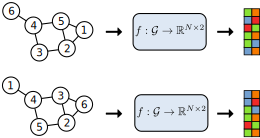
\includegraphics[width=.8\textwidth]{equivariant}
  \end{center}
\end{frame}

\begin{frame}{Graphs versus Images  \unfootnote{Inspired by M. M. Bronstein}}

  \begin{columns}
    \begin{column}{0.45\textwidth}
      \begin{center}
        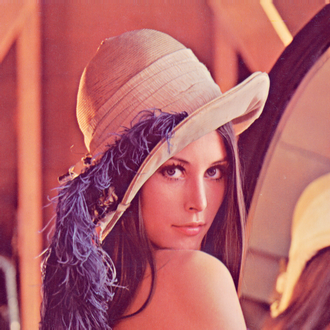
\includegraphics[width=0.5\textwidth]{lenna}
      \end{center}
      \begin{itemize}
      \item Constant number of neighbours
      \item Fixed position of neighbours
      \item We want shift invariance
      \end{itemize}
    \end{column}
    \begin{column}{0.55\textwidth}
      \begin{center}
        
\includegraphics[width=0.5\textwidth]{simple_graph}
      \end{center}
      \vspace{1cm}
      \begin{itemize}
      \item Variable number of neighbours
      \item No predefined ordering of neighbours
      \item Permutation (equi/in)variance
      \end{itemize}
    \end{column}
  \end{columns}
\end{frame}

\begin{frame}{A first problem}
  \begin{definition}[Graph Isomorphism]
    $G_1 = (V_1,E_1) \simeq G_2 = (V_2,E_2)$ iff it exists a bijection
    $f:V_1 \to V_2$ s.t. $(u,v) \in E_1 \Leftrightarrow (f(u), f(v))
    \in E_2$.
  \end{definition}


  \begin{block}{Remarks}
    \begin{itemize}
    \item Notion of ``Equality'' between graphs.
    \item NP-Intermediate problem
    \item Labeled version : $l_v(u) = l_v(f(u)), \forall u \in V_1$
    \end{itemize}
  \end{block}
\end{frame} 

\begin{frame}[plain]
  \begin{center}
    \begin{huge}
      How to adapt CNN to Graphs ?
    \end{huge}

    \vfill
    How to adapt convolution and pooling to variable dimension and
    permutation ?
  \end{center}
\end{frame}

\section{GNN}
\subsection{Historical tentatives}
%% \begin{frame}{A timeline}
%%   \begin{columns}
%%     \begin{column}{0.45\textwidth}
%%       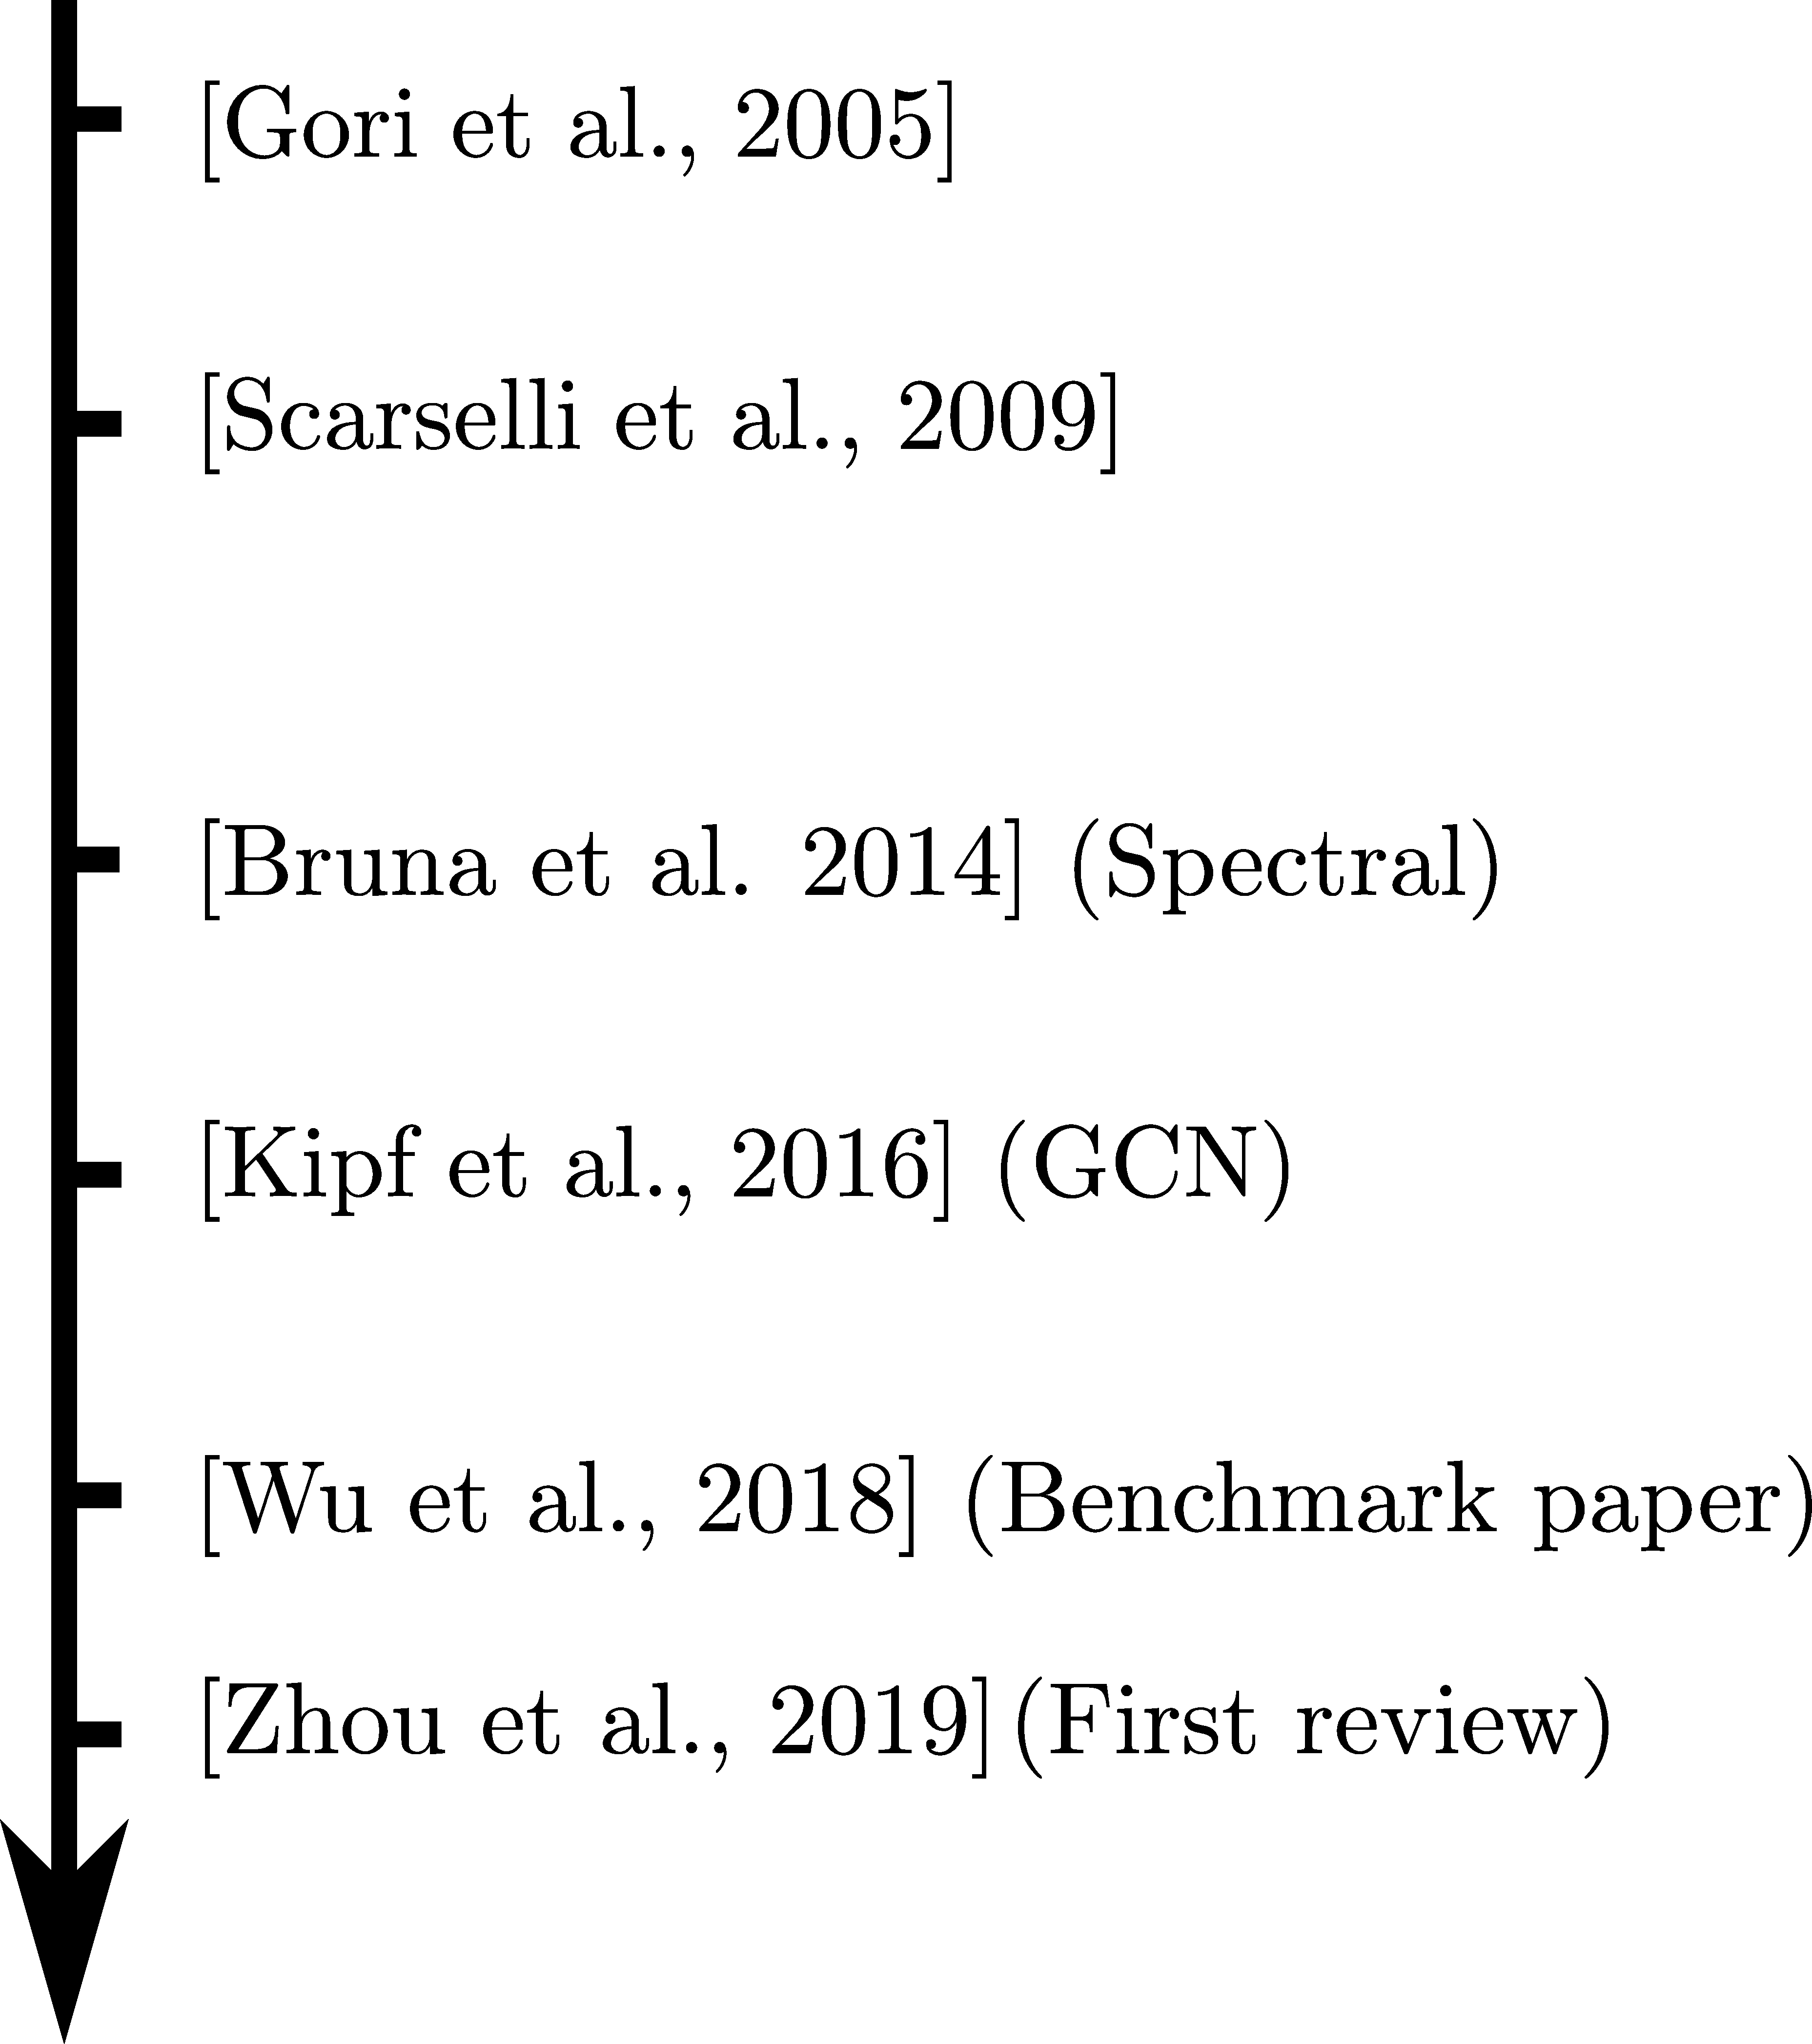
\includegraphics[height=.7\textheight]{gnn_timeline}
      
%%     \end{column}
%%     \begin{column}{0.6\textwidth}
%%       \begin{itemize}
%%       \item First attempt before Deep Era
%%         \vfill
%%       \item Explosion of papers since 2018
%%         \vfill
%%       \item See Sergey's analysis
%%       \end{itemize}
%% \centering{      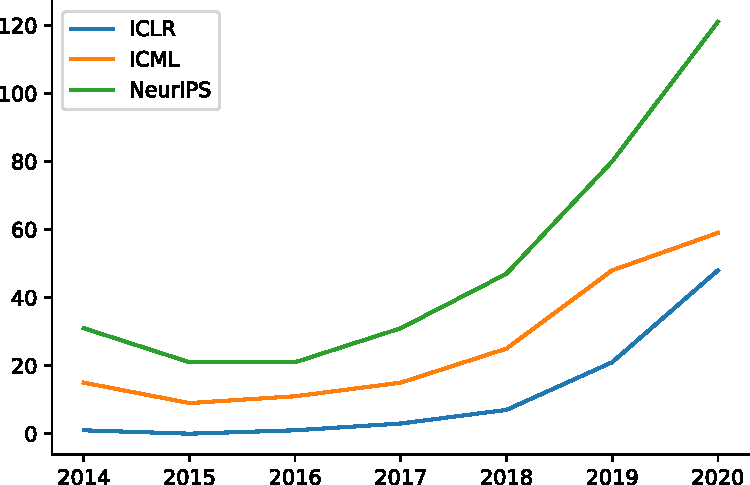
\includegraphics[width=.7\textwidth]{data_papers_graph.pdf}
%%       }\flushright{{\scriptsize [data source: dplb]}} 
%%     \end{column}
%%   \end{columns}
%% \end{frame}

\subsection{Message passing framework}
\begin{frame}{Message passing framework}
  \framesubtitle{An introduction}
  \begin{block}{Intuition}
    Update node representation according to neighbours
    \begin{center}
      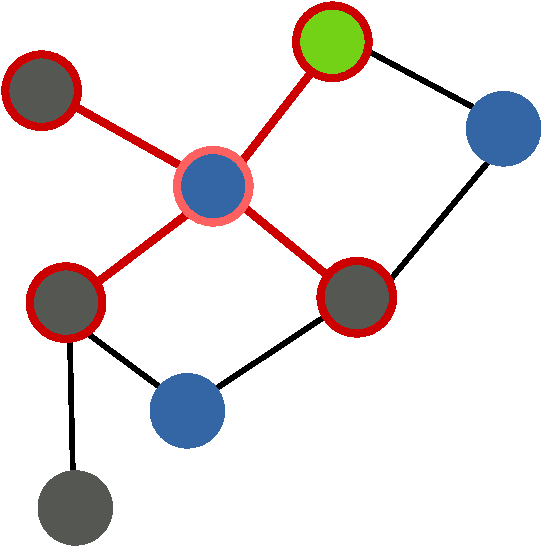
\includegraphics[height=0.5\textheight]{mpnn_1}
    \end{center}
  \end{block}
    
\end{frame}
\begin{frame}{General principle}
  \begin{center}
    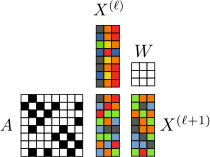
\includegraphics[width=\textwidth]{mpnn_2}
  \end{center}

\end{frame}

\begin{frame}{Convolutions on graphs}
  % \begin{columns}
  %   \begin{column}{0.5\textwidth}
      \begin{itemize}
      \item $A$ : Adjacency Matrix
      \item $AX^{(\l)}(i,:)$ : Sum all informations of $\mathcal{N}(v_i)$
      \item $AX^{(\l)}(i,:)W = X^{(\l+1)}$ : ``nearly'' updated feature of $v_i$
      \end{itemize}
      \vfill
    % \end{column}
    % \begin{column}{0.5\textwidth}
\centering{          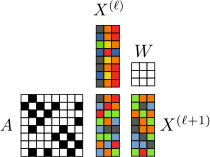
\includegraphics[width=.5\textwidth]{mpnn_2}
}  %   \end{column}
  % \end{columns}
\end{frame}

\begin{frame}{Message passing framework \unfootnote{\cite{Gilmer2017}}}
  \begin{block}{Message}
    \begin{itemize}
    \item Aggregate all information of neighboorhood%of each $v_i$
      % trough $f$
    \item $m_i^{(\l+1)} = \sum_{v_j \in \mathcal{N}(v_i)}
      f(X^{(\l)}_i,X^{(\l)}_j,e_{i,j})$

    \item $AX(i,:) = \sum_{v_j \in \mathcal{N}(v_i)} X(j,:)$
    \end{itemize}
  \end{block}
  \begin{block}{Update}
    \begin{itemize}
    \item Compute the new representation $X^{(\l+1)}$
    \item $X_i^{(\l+1)} = g(X_i^{(\l)}, m_i^{(\l+1)})$
    \item $X^{(\l+1)} (i,:) = \sigma(AX^{(\l)} (i,:)W + X^{(\l)} (i,:))$
    \item $\sigma(\cdot)$ : non linear activation function (ReLU).
    \end{itemize}
  \end{block}
\end{frame}

\begin{frame}{MPNN Layer}

  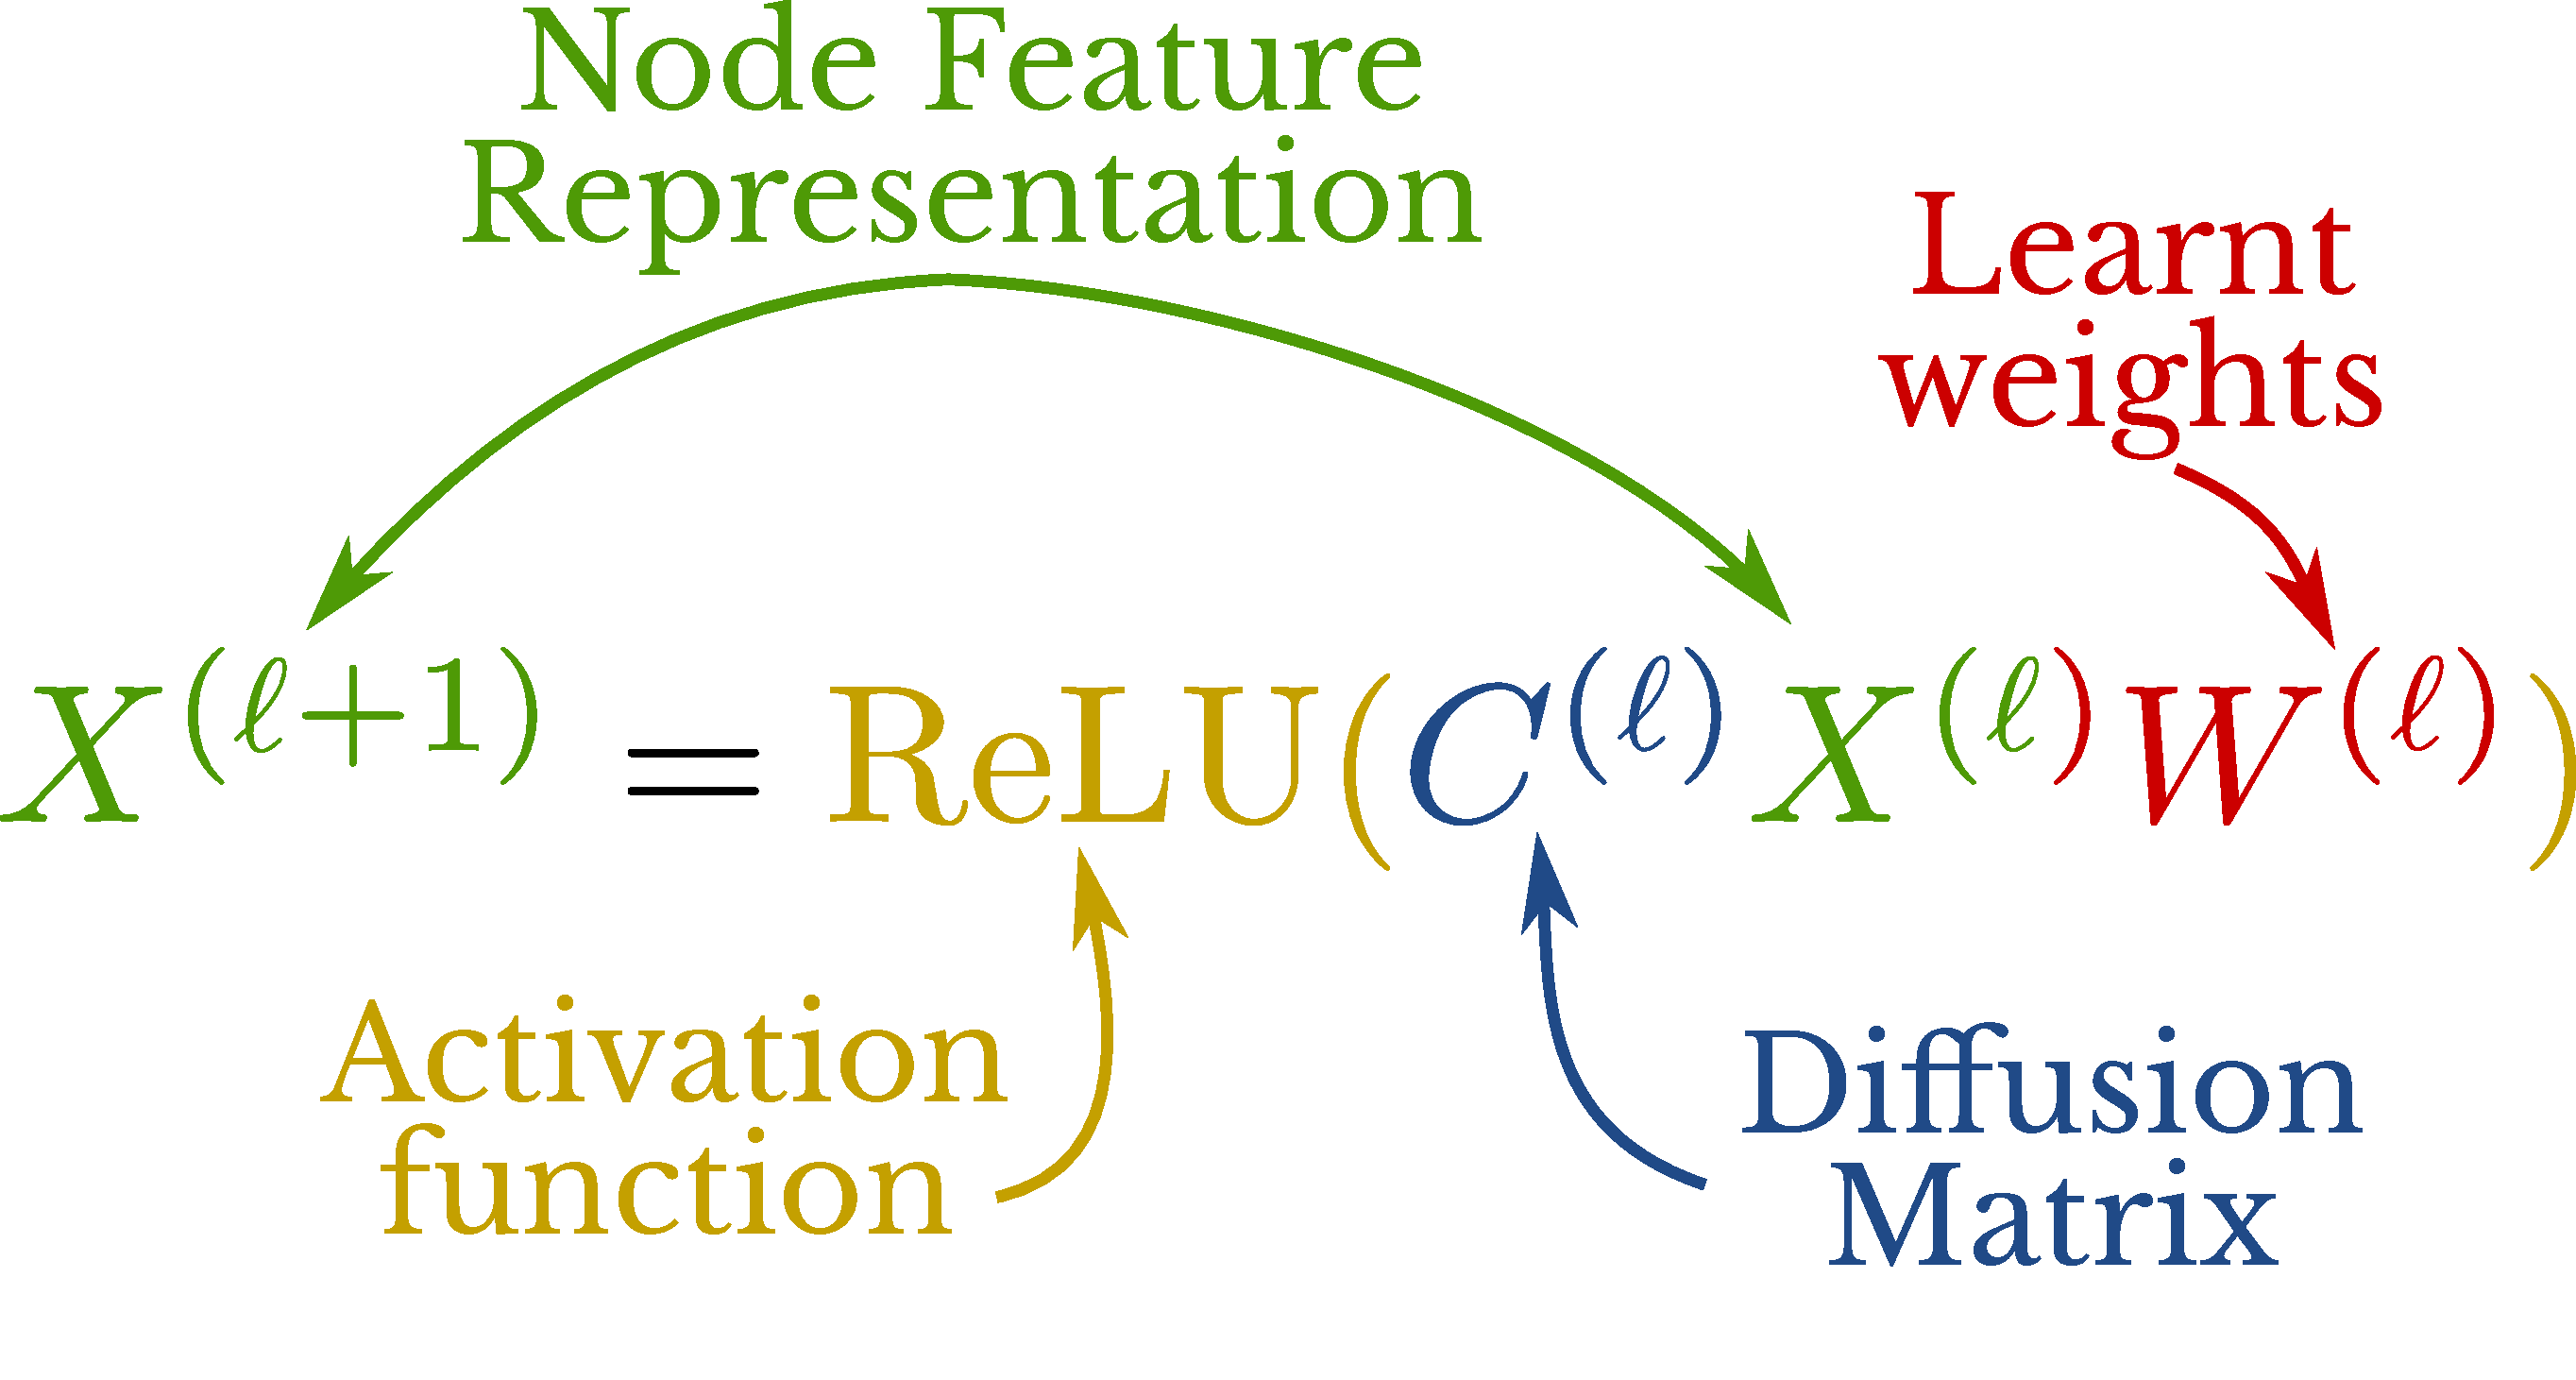
\includegraphics[width=\textwidth]{mpnn_equation}
  
\end{frame}




% \subsection{Spectral approach}

% \begin{frame}{Spectral approach}
%   \begin{block}{Spectral theory}
%     \centering{{\huge $$L = D - A$$}}
%     \begin{itemize}
%     \item Normalized version: $\tilde{L} = I - D^{-\frac{1}{2}} A
%       D^{-\frac{1}{2}}$ 
%     \item Measure the smoothness of a signal $\s$ on a graph:
%       $$\s^\top L\s = \sum_{(u,v) \in E} (\s(u) - \s(v))^2 $$
%     \end{itemize}
%   \end{block}
% \end{frame}

% \begin{frame}{Spectral convolutions}
%   \begin{block}{Laplacian decomposition}
%     \begin{itemize}
%     \item $L = U \Lambda U^\top$
%     \item  $\Lambda(i,i) = \lambda_i $ : i-th eigenvalue of $L$
%     \item Filtering a signal $\s$:
%       $$\s' = U\Phi(\Lambda)U^\top \s$$
      
%     \end{itemize}
%   \end{block}
%   \begin{block}{Spectral convolution}
%     \begin{itemize}
%     \item Apply a transformation on $\Lambda$
%     \item 
%     \end{itemize}
%   \end{block}
% \end{frame}

% \begin{frame}
%   a laisser à muhammet
% \end{frame}


\subsection{Beyond MPNN}
\begin{frame}{Graph Attention Networks\unfootnote{\cite{Velickovic2017}}}
  \begin{block}{MPNN }
    \begin{itemize}
    \item MPNN considers all neighboors in the same way
    \item Isotropic aggregation
    \item $\Rightarrow$ over-smoothing of information
    \end{itemize}
  \end{block}
  \begin{block}{Bringing attention to MPNN}
    \begin{itemize}
    \item Weight each contribution of neighboor differently
     $$m_i^{\l+1} = \sum_{v_j \in \mathcal{N}(v_i)}\emph{
       \alpha_{i,j}} X(j,:)$$
     
   \item $\alpha_{i,j}$ : attention coefficient
    \end{itemize}
    
  \end{block}
\end{frame}

\begin{frame}{Graph Attention Networks}
  \begin{block}{Attention coefficient} 
    \begin{center}
      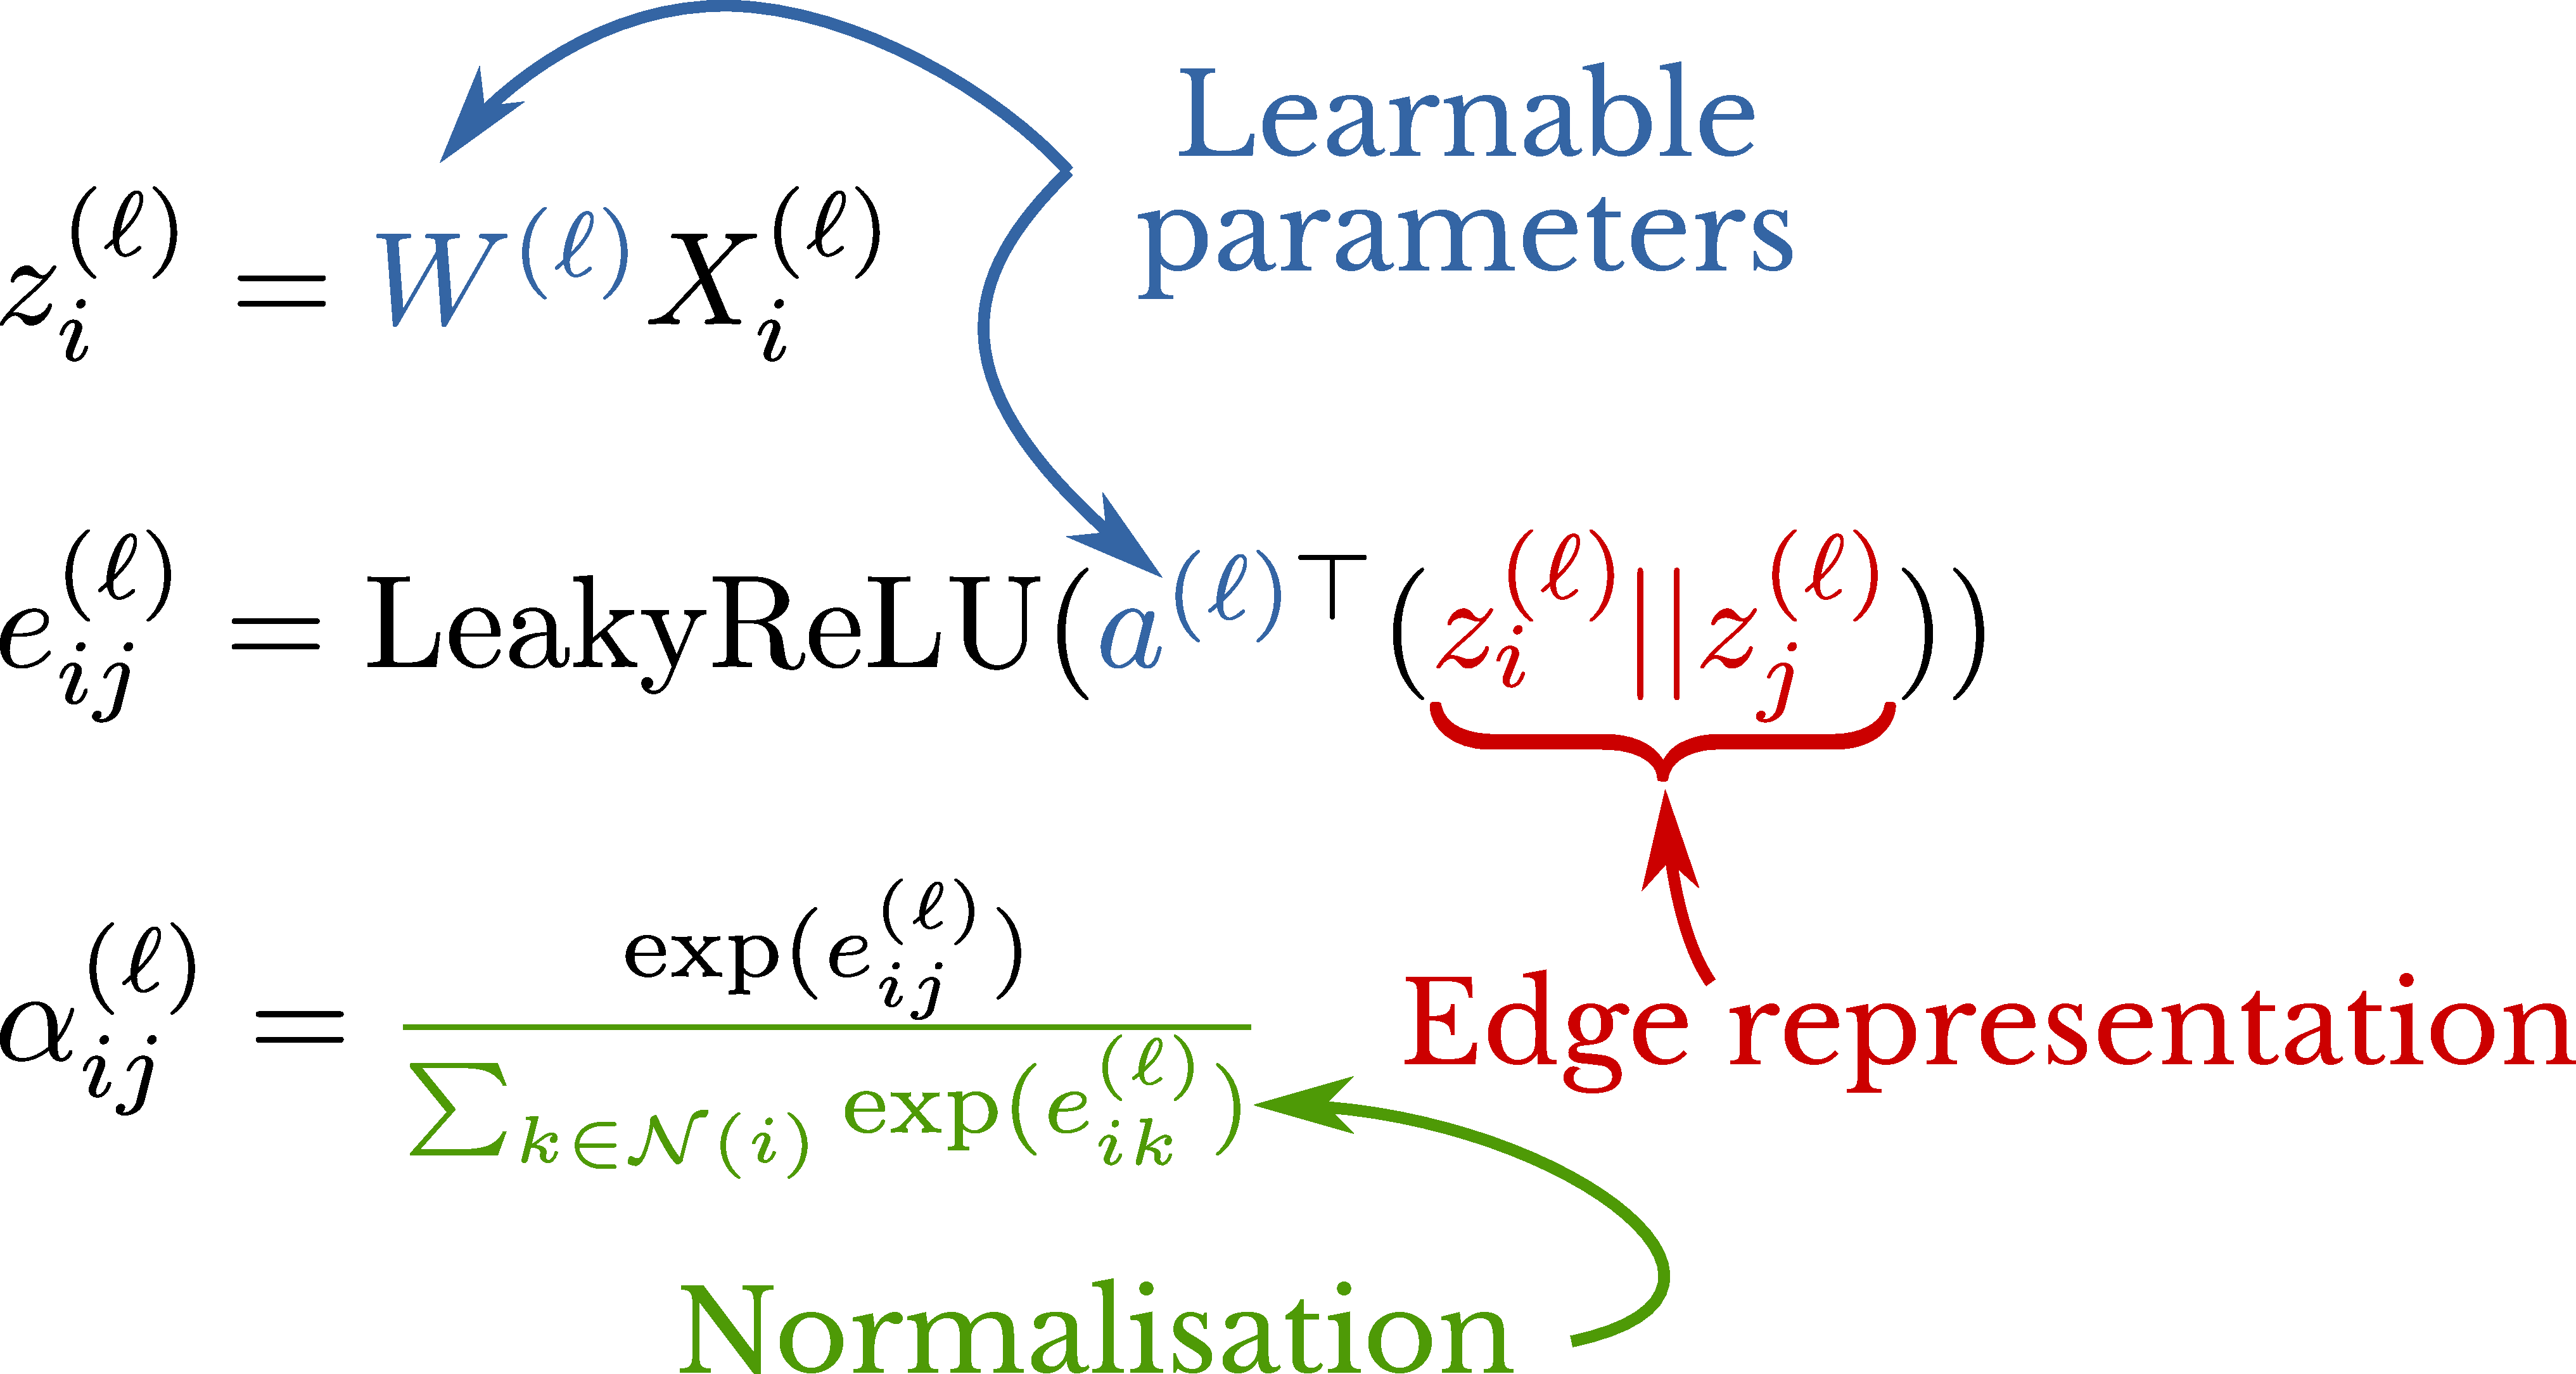
\includegraphics[width=.8\textwidth]{gat}
    \end{center}
  \end{block}
  
\end{frame}


\begin{frame}{Graph Attention Networks}
  \begin{center}
    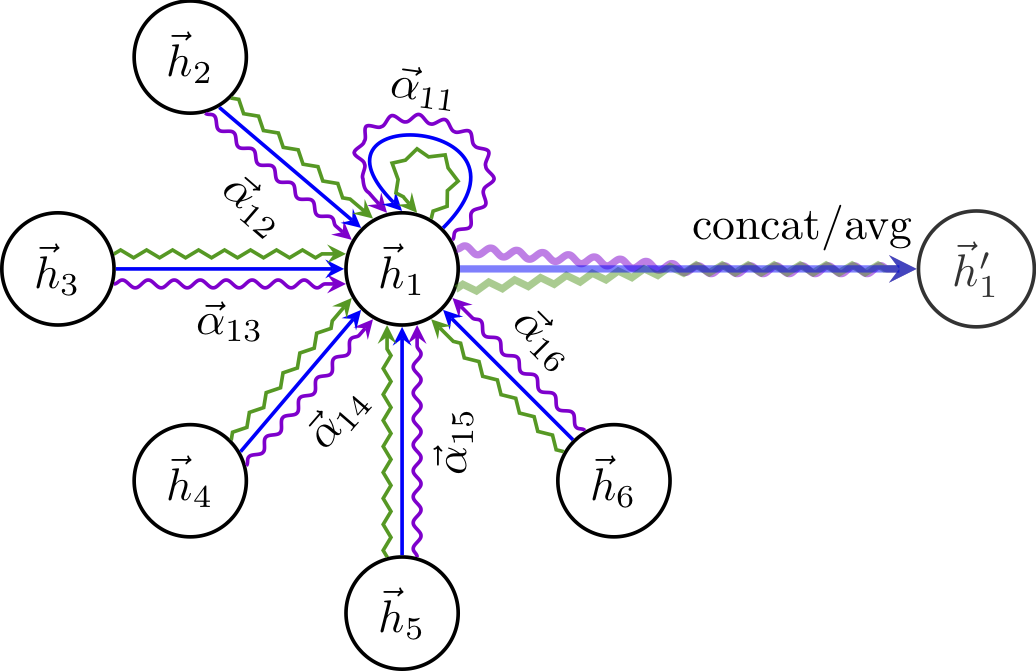
\includegraphics[width=\textwidth]{gat_velik}
  \end{center}
  \flushright{\url{https://github.com/PetarV-/GAT}}

  
\end{frame}

\begin{frame}{MPNN family}
  \begin{block}{Node Representation Learning}
    \begin{itemize}
    \item Build representation for nodes
    \item Useful for node level tasks
    \item Not complete for graph level
    \end{itemize}
    \begin{center}
      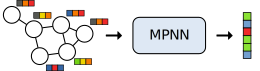
\includegraphics[width=\textwidth]{node_level}
    \end{center}
  \end{block}
\end{frame}


\begin{frame}{Read Out}
  \begin{center}
    \Huge{ How to transform node representation to graph representation ?}
  \end{center}
\end{frame}

\begin{frame}{Aggregation step}
  \begin{block}{Readout function}
    $$
    \hat{y} = R(\{X_i^{(\L)} |  v_i \in V \})
    $$
  \end{block}
  \uncover<2>{
    \begin{itemize}
    \item Differentiable
    \item Permutation invariant
      
    \item Simple statistics : mean, sum.
    \item Learnable : \cite{Ying2018}
    \end{itemize}
    \vfill
    \begin{center}
      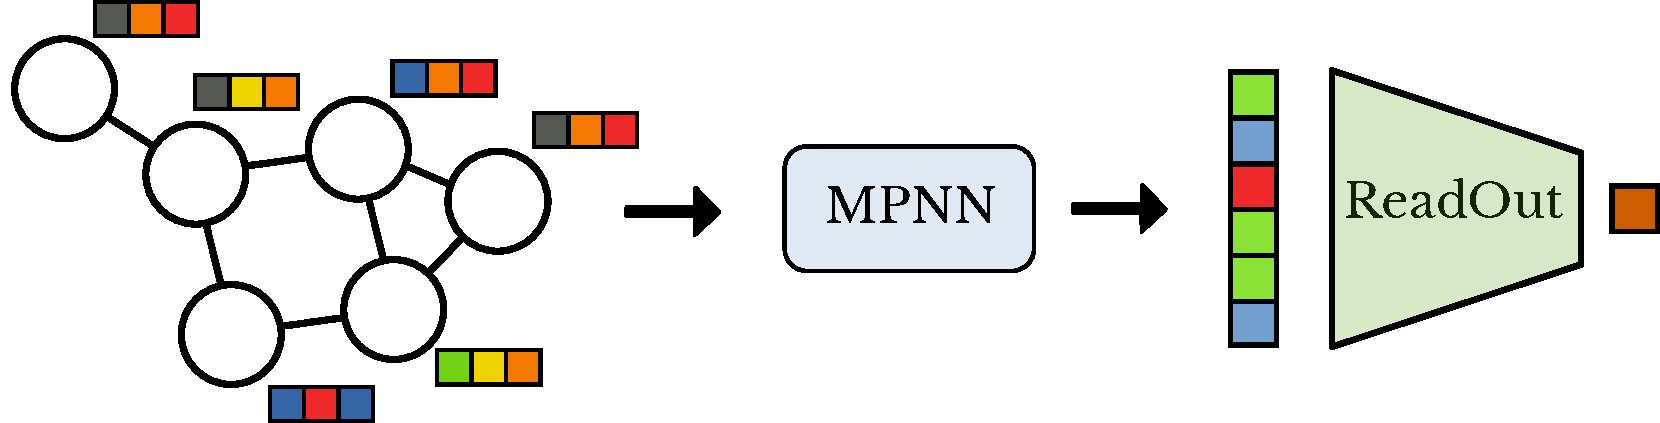
\includegraphics[width=.9\textwidth]{graph_level}
    \end{center}
  }
  
\end{frame}


\begin{frame}{DiffPool\unfootnote{\cite{Ying2018}}}
  \begin{center}
    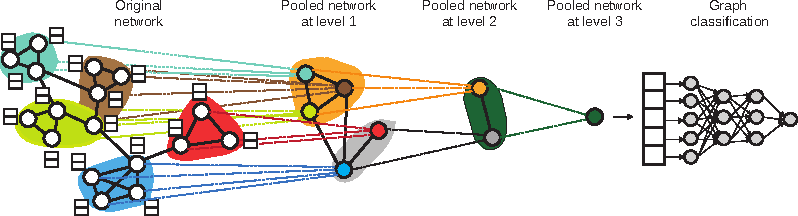
\includegraphics[width=\textwidth]{diffpool} \flushright \tiny{taken
      from \cite{Ying2018}}
  \end{center}

  \begin{block}{Aggregation level}
{\small     \begin{itemize}
    \item Learnt Cluster Assignment Matrix $S^{(\l)} \in \dbR^{n_l \times n_{l+1}}$
    \item Node representation : $X^{(\l+1)} = S^{(\l)\top} X^{(\l)}$
    \item Adjacency matrix : $A^{(\l+1)} = S^{(\l) \top} A^{(\l)} S^{(\l)}$
    \end{itemize}
}    
  \end{block}

\end{frame} 


\begin{frame}{Graph Networks\unfootnote{\cite{Battaglia2018}}}

  \begin{block}{Generalize MPNN}
    \begin{itemize}
    \item Theoretical framework
    \item Three levels of representations:
      \begin{enumerate}
      \item Edge $ \e_{ij}$
      \item Node $X_i$ or $\h_i$
      \item Graph $ \z$
      \end{enumerate}
    \item[$\Rightarrow$] Three pairs of message/update functions
    \item Introduce edge representation learning
    \end{itemize}
    
  \end{block}

  \begin{center}
    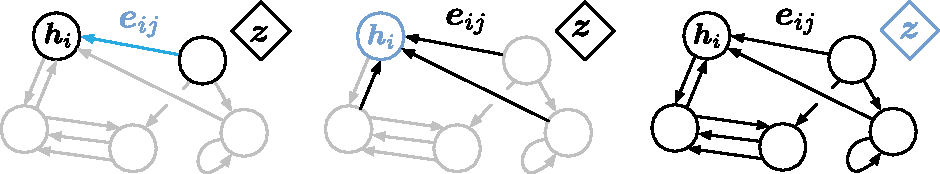
\includegraphics[width=\textwidth]{gn}
    \flushright{{\scriptsize taken from \cite{Battaglia2018}}}
  \end{center}
  
    
\end{frame}


\begin{frame}{Edge representation}

 
    \begin{center}
      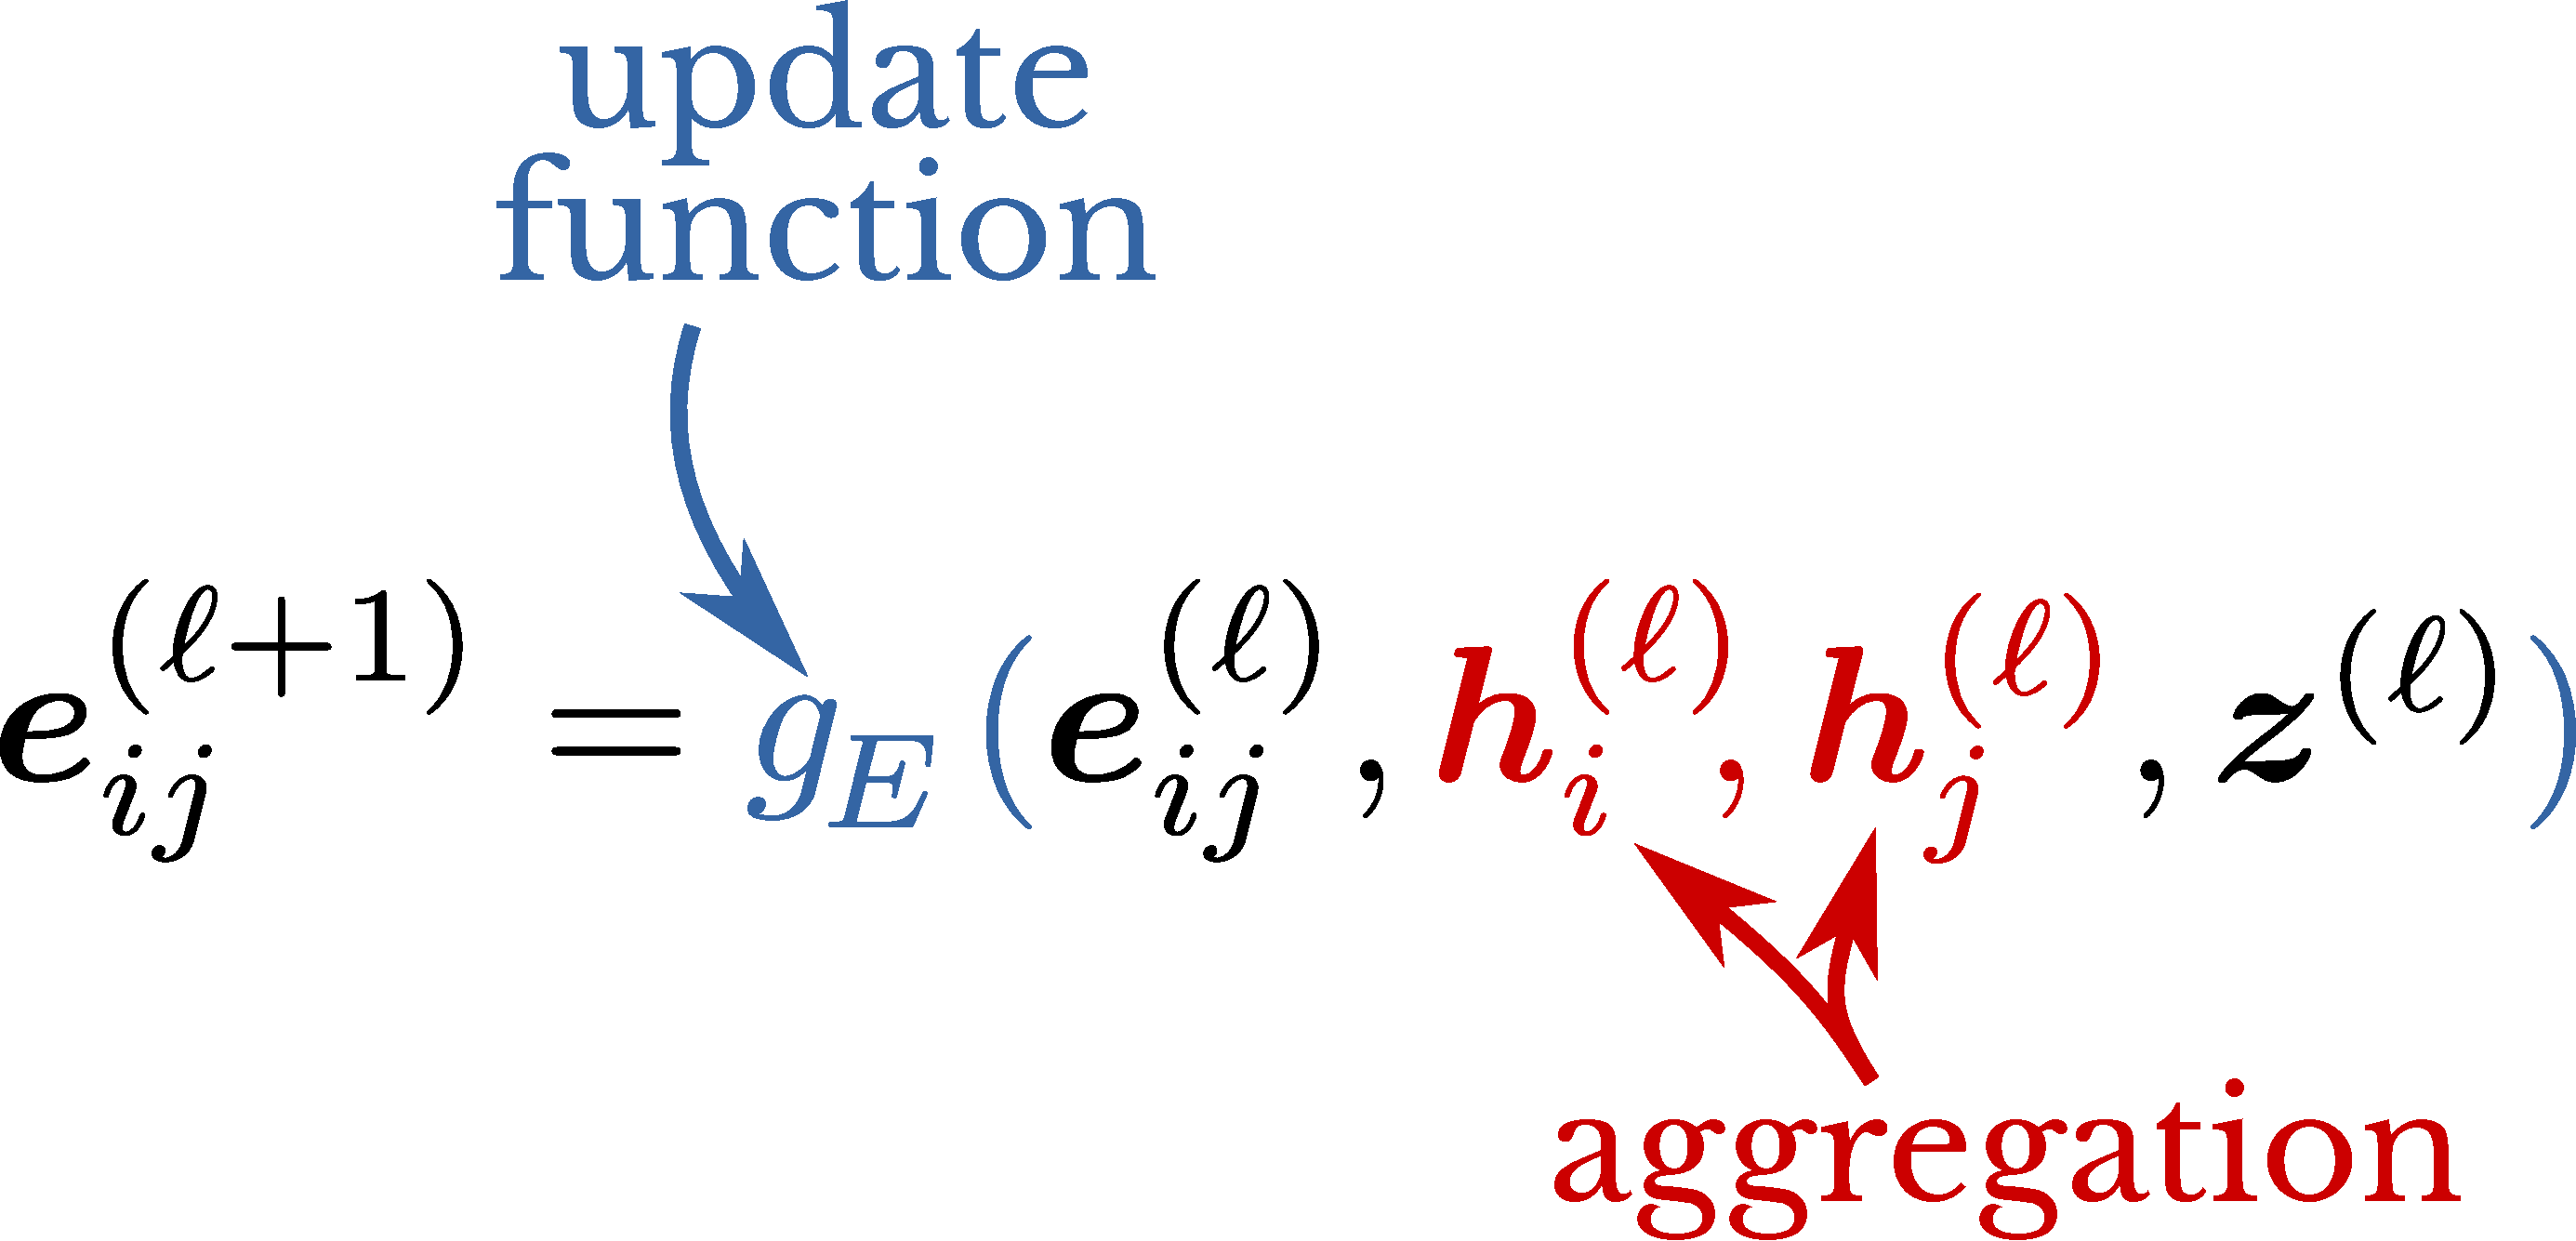
\includegraphics[width=\textwidth]{eij_gn}
    \end{center}
    \flushright{{\scriptsize $\rightarrow$ See Guillaume's presentation for an implementation}}
\end{frame}


\begin{frame}{Node representation}
  
    \begin{center}
      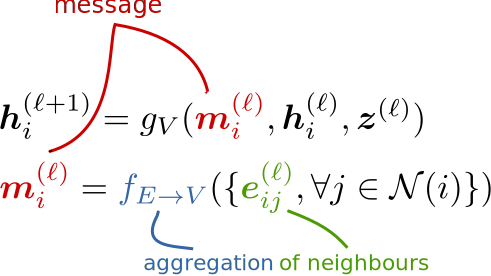
\includegraphics[width=\textwidth]{hi_gn}
    \end{center}
\end{frame}

\begin{frame}{Graph representation}
  
    \begin{center}
      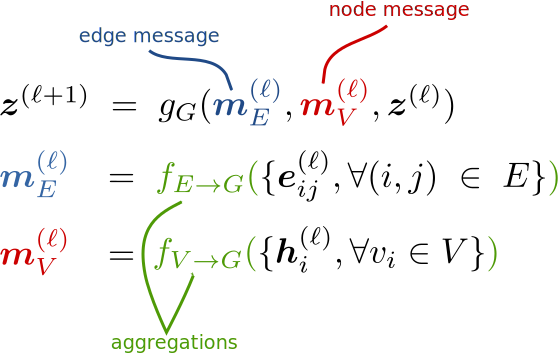
\includegraphics[width=\textwidth]{z_gn}
    \end{center}
\end{frame}


\begin{frame}[allowframebreaks]{Theoretical aspects}
  \begin{block}{Interpretability: How to evaluate GNN ? }
    \begin{itemize}
    \item Determine if a GNN can distinguish two graphs
    \item $GNN : \mathcal{G} \to \R^{d \times N}$
    \item $G_1 \simeq G_2 \Leftrightarrow GNN(G_1) = GNN(G_2)$ ?
    \end{itemize}
  \end{block}
  \break

{\small   \begin{block}{Relationship with Weisfeler-Lehman test}
    \begin{itemize}
    \item Iterative coloring process
    \item Polynomial approximation of isomorphism
    \item ``classic'' GCNs $\leq$ WL-Test
    \item Higher order of WL-test exist
    \end{itemize}
  \end{block}
}  \centering{  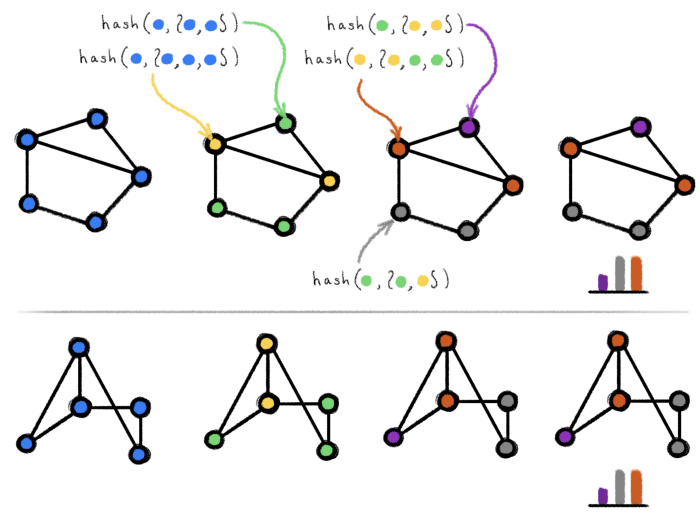
\includegraphics[width=.4\textwidth]{wl-bromstein}}
  \flushright{{\tiny M. Bronstein, medium blog}}
  
\end{frame}



\begin{frame}{Limitations of GNNs}
  \begin{block}{Low pass filtering}
    \begin{itemize}
    \item Each iteration aggregates the neighboor's information
    \item Aggregation is (usually) isotropic
    \item Extend to not only low pass : spectral approaches\\
      \flushright{\scriptsize $\rightarrow$ See Muhammet's talk}
    \end{itemize}
  \end{block}
  \begin{block}{Over smoothing}
    \begin{itemize}
    \item Adding layers increases smoothing
    \item At one point: all node's info is shared 
    \item No real \emph{deep} networks: generally 2 layers
    \end{itemize}
  \end{block}
\end{frame}

% \begin{frame}{Relationship with Transformers}
%   %https://thegradient.pub/transformers-are-graph-neural-networks/
%   \begin{block}{Transformers}
    
%   \end{block}
%   \begin{block}{GNN generalize Transformers}
    
%   \end{block}
% \end{frame}

\section{Graph Generation}
\begin{frame}{Graph generative models}
  \begin{block}{Graph generation}
    \begin{itemize}
    \item Create new graphs
    \item $f : \R^d \to \mathcal{G}$
    \item Explore latent euclidean space
    \end{itemize}
  \end{block}
  \begin{block}{Application}
    \begin{itemize}
    \item Drug discovery
    \item Generate new molecules with particular properties 
    \end{itemize}
  \end{block}
  \begin{center}
    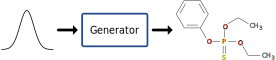
\includegraphics[width=.8\textwidth]{graph_generator}
  \end{center}
\end{frame}


\subsection{Graph Auto Encoders}

\begin{frame}{Graph Auto Encoders}
  \begin{columns}
    \begin{column}{.5\textwidth}
      \textbf{Encoder}
      \begin{itemize}
      \item GNN 
      \end{itemize}
      $$Z = \textrm{enc}_\Phi(A)$$
      
    \end{column}
    \begin{column}{.5\textwidth}
      \textbf{Decoder}
      \begin{itemize}
      \item Reconstruct Adjacency matrix
        $$\hat{A}(i,j) = \sigma(\z_i^\top \z_j)$$
      \end{itemize}
      
    \end{column}
  \end{columns}
  \centering{
    \textbf{Problem}
    $$
    \min_{\Phi} \sum_{i=1}^N \| A(i,:) - \hat{A}(i,:)\|^2
    $$
  \vfill

  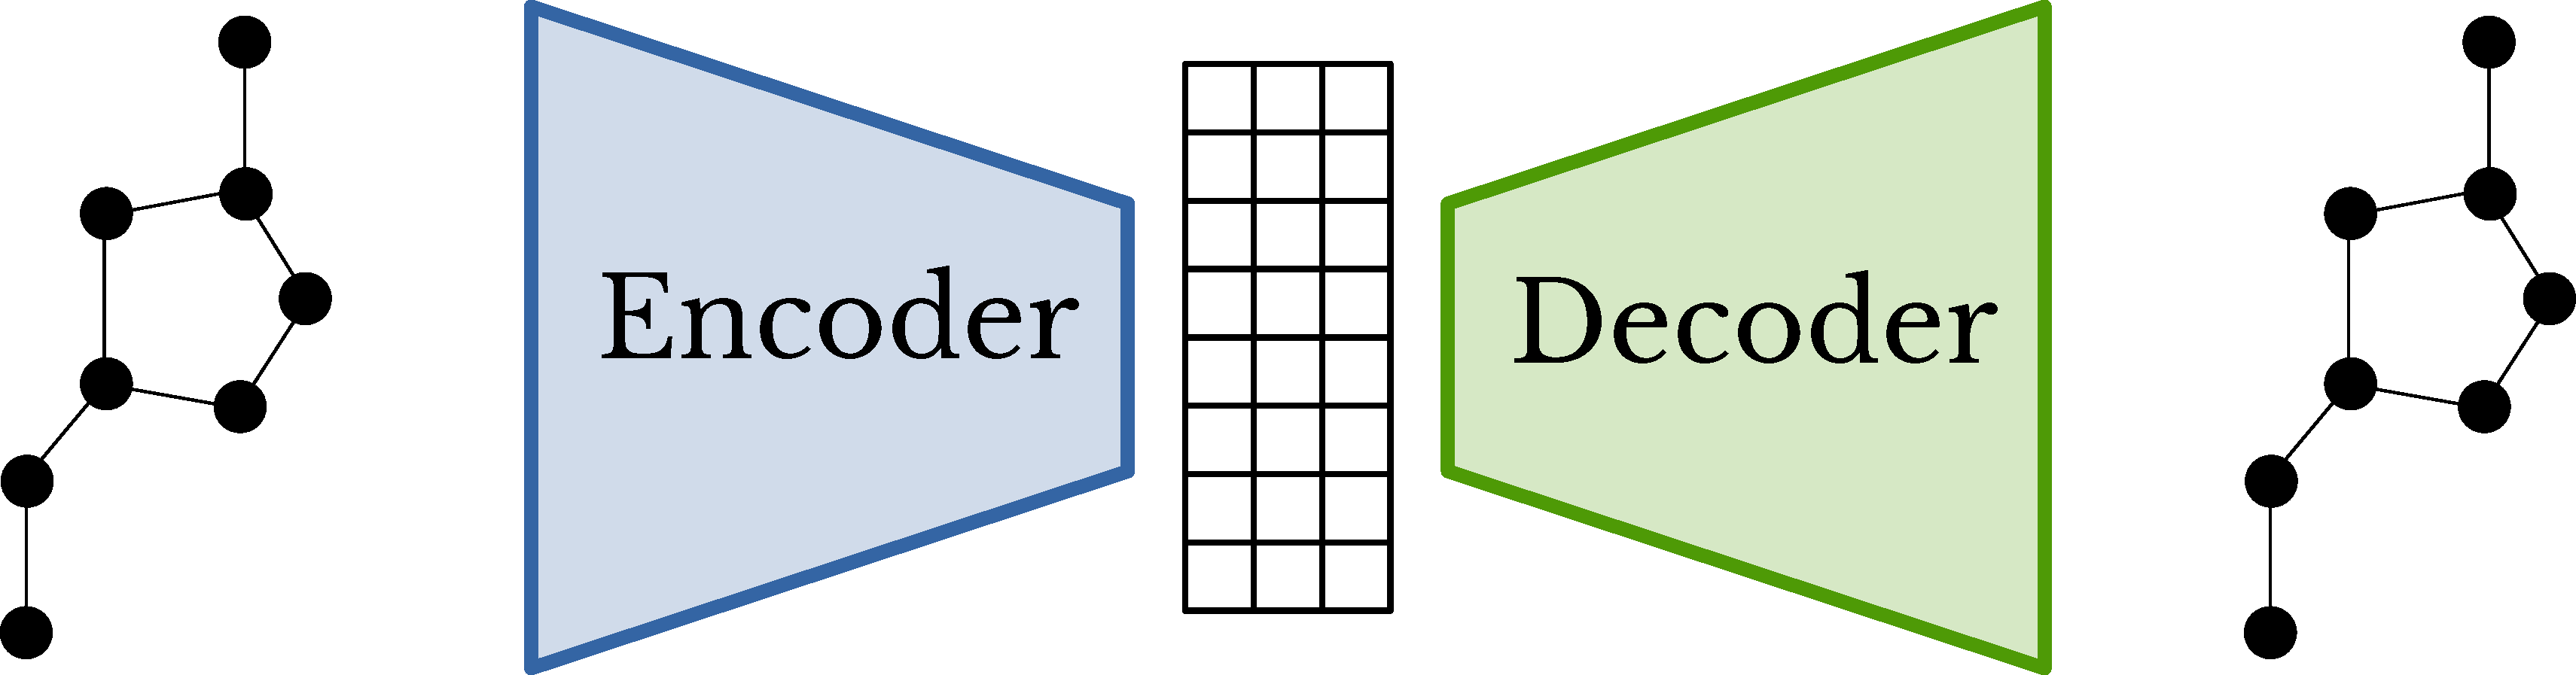
\includegraphics[width=.8\textwidth]{vae}}
\end{frame}

\begin{frame}{Other graph generation approaches}
  \begin{columns}
    \begin{column}{.6\textwidth}
      \begin{itemize}
      \item Variationnal auto encoders\\ (KL divergence)
      \item GANs
      \item Reinforcement learning
      \item Recursive processes
      \end{itemize}
    \end{column}
    \begin{column}{0.4\textwidth}
      \flushright{\scriptsize \cite{DeCao2018}}
      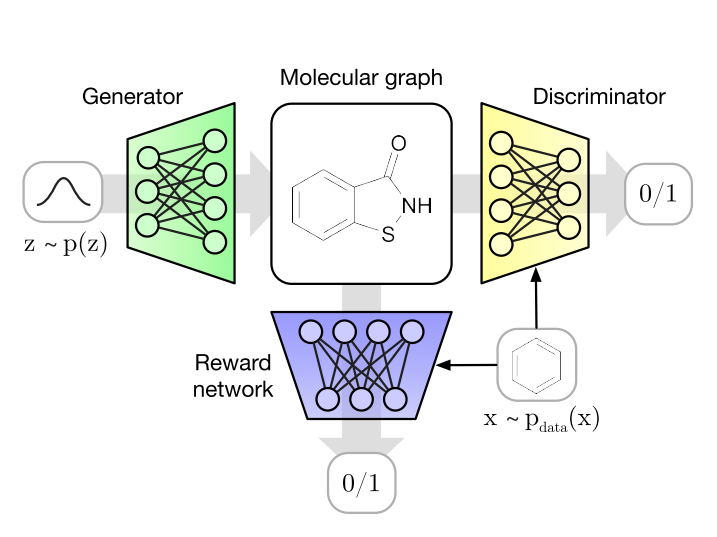
\includegraphics[width=\textwidth]{molgan_overview}
      
    \end{column}
  \end{columns}
  \vfill
\centering{  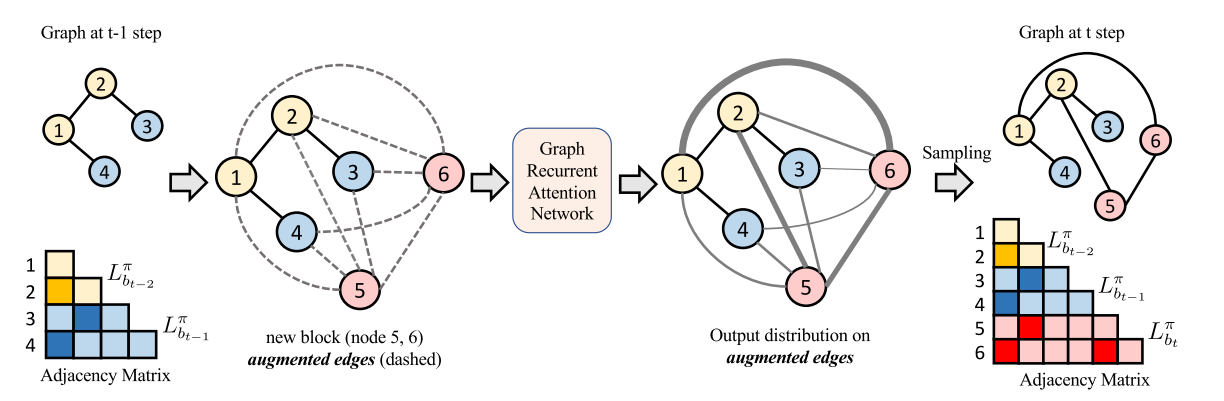
\includegraphics[width=.7\textwidth]{autoregressive} 
}
\flushright{\scriptsize \cite{Liao2019}}
  
\end{frame}

\section{Application and Evaluation}
\subsection{Datasets}

\begin{frame}{Application domains of GNN}
  \begin{block}{Node level prediction}
    \begin{itemize}
    \item Citation networks
    \item Node Clustering
    \end{itemize}
  \end{block}

  \begin{block}{Link prediction}
    \begin{itemize}
    \item Collaboration graphs
    \item Knowledge graphs
    \item Temporal graphs
    \item Recommandation
    \end{itemize}
  \end{block}

  \begin{block}{Graph prediction}
    \begin{itemize}
    \item Molecular property prediction
      \begin{itemize}
      \item Physiologic, toxicity, physical, quantum mechanics \dots
      \end{itemize}
    \item Protein-Protein interactions
    \item Programs, source code
    \end{itemize}
  \end{block}
\end{frame}
\begin{frame}{Emergence of datasets}
  \begin{block}{The rise of Deep Learning in Computer Vision}
    \begin{itemize}
    \item 3 causes :
      \begin{itemize}
      \item Number of layers
      \item Computationnal power
      \item Datasets
      \end{itemize}
    \item Standardized big datasets
    \item MNIST, ImageNet, CIFAR, \dots
      \vfill
      \centering{
        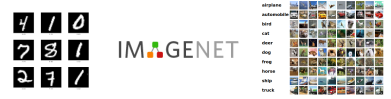
\includegraphics[width=\textwidth]{datasets}
        
      }
    \end{itemize}
  \end{block}
\end{frame}

\begin{frame}[allowframebreaks] {Datasets for Graph Machine Learning}

 
  \begin{center}
    
\includegraphics[width=.4\textwidth]{OGB}
  \end{center}

  \begin{columns}
    \begin{column}{.42\textwidth}
      {\small       \begin{itemize}
        \item\url{ogb.stanford.edu}
        \item 15 datasets
        \item Molecular graphs, citation networks,\dots
        \end{itemize}
      }
    \end{column}
    \begin{column}{.58\textwidth}
      \centering{
        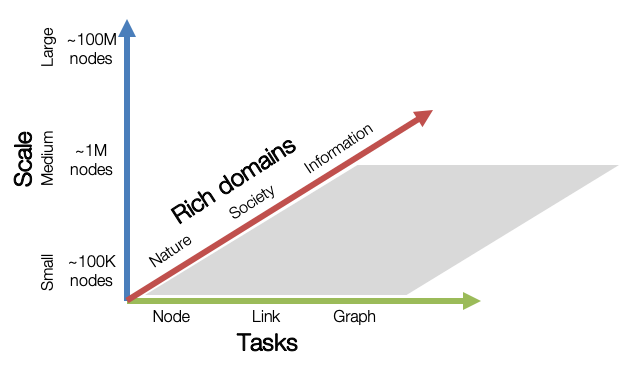
\includegraphics[width=\textwidth]{ogb_overview}
      }
      
    \end{column}
  \end{columns}
    
  \break
  \centering{
    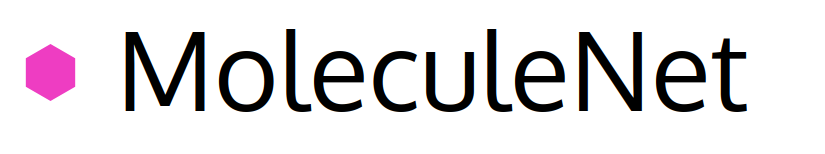
\includegraphics[width=.6\textwidth]{moleculenet}

    \vspace{.3cm}
    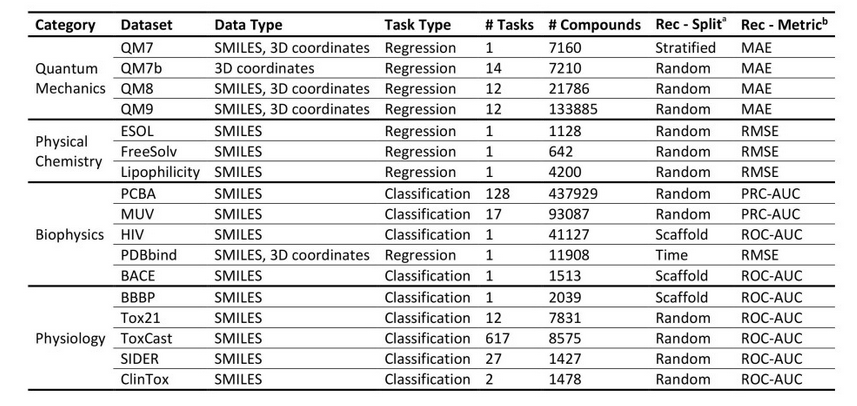
\includegraphics[width=\textwidth]{moleculenet_overview}

  }
  
\flushright{\scriptsize{\url{moleculenet.ai}}}

\break

  \begin{block}{MOSES}
    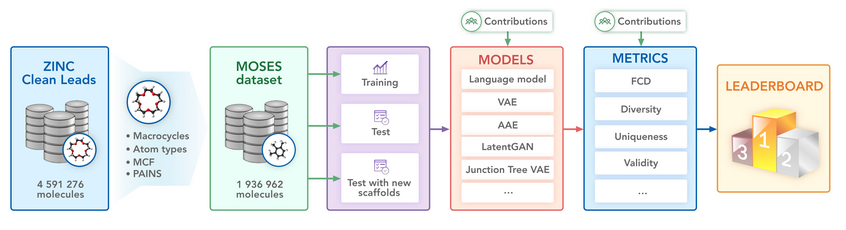
\includegraphics[width=\textwidth]{moses}
    \begin{itemize}
    \item \url{https://github.com/molecularsets/moses}
    \item Dataset for generative models 
    \end{itemize}
  \end{block}
\end{frame}

\begin{frame}{Conclusion and Outlooks}

  \begin{block}{GNNs}
    \begin{itemize}
    \item Bring representation learning to graphs
    \item Dynamic and growning field
    \item Still in infancy, but supported by industry
    \item Still some limitations
      \begin{itemize}
      \item Still computes a Euclidean embedding
      \item Not deep yet
      \end{itemize}
    \end{itemize}
  \end{block}

  \begin{block}{Outlooks}
    \begin{itemize}
    \item Dynamic graphs
    \item Interpretability
    \item Real ``Deep'' Learning ?
    \item Improve readout ? is it useful ?  
    \end{itemize}
  \end{block}
\end{frame}

\begin{frame}{Questions and Discussion}
  \begin{columns}
    \begin{column}{.6\textwidth}
  {\Large
    \begin{itemize}
    \item Possible use of GNN ?
    \item How to find our place ?
    \item Collaborations ?
    \end{itemize}
  }
      
    \end{column}
    \begin{column}{.4\textwidth}\centering{
      
\includegraphics[height=.4\textheight]{question_mark}}
    \end{column}
  \end{columns}
\end{frame}


% =================================================================================
\nocite{*}
\begin{frame}[allowframebreaks]
  \frametitle{References}
      \bibliographystyle{plainnat}
      \bibliography{biblio_gnn}
\end{frame}



\end{document}
